\documentclass[a4paper,11pt]{article}
\usepackage[T1]{fontenc}
\usepackage[utf8]{inputenc}
\usepackage{lmodern}
\usepackage{mathptmx}
\usepackage[margin=2.5cm]{geometry}
\usepackage{makeidx}
\usepackage{setspace}
\usepackage{fancyhdr}
\usepackage{lastpage}
\usepackage{graphicx}
\usepackage{amsmath}
\usepackage{makeidx}
\usepackage[utf8]{inputenc}
\usepackage[spanish]{babel}
\makeindex 
\graphicspath{{../imagenes/}}                                % Setea el path de las imagenes
\pagestyle{fancy}
\fancyhf{}
\renewcommand{\headrulewidth}{0pt}                        % Saca la línea horizontal del borde superior de las páginas
\cfoot{Pág. \thepage \hspace{1pt} de \begin{NoHyper}\pageref{LastPage}\end{NoHyper}}  % Escribe la cantidad de paginas en el pie de página
\makeindex                                                % Crea el índice
\onehalfspacing                                           % Setea un punto y medio de separación entre líneas
\setlength{\parskip}{6pt}                                 % Setea 6 puntos de separación entre párrafos
\renewcommand{\figurename}{Figura}
\renewcommand\refname{Referencias}
\renewcommand\contentsname{Índice}
\usepackage{hyperref} % For hyperlinks in the PDF
\usepackage{csquotes}
\usepackage[backend=bibtex,bibencoding=ascii, style=alphabetic-verb]{biblatex}
\bibliography{bibliografia}

\title{}
\author{}

%Ésto está echo?
%Títulos de capítulo: Arial ó Times New Roman, 14 puntos, negrita.
%Subtítulos dentro de cada capítulo: Arial ó Times New Roman, 12 puntos, negrita (opcional:
%subrayado). (pueden ir numerados).

\begin{document}


  % ############################ INICIO CARATULA ############################

  \begin{titlepage}

    \begin{center}

      \begin{Huge}
        \textbf{Facultad de Ciencias Exactas, Ingenieria y Agrimensura}\\  
      \end{Huge}
      \vspace*{0.5in}
      \begin{huge}
        \textbf{Licenciatura en Ciencias de la Computación}\\
      \end{huge}
      \vspace*{0.5in}
      \begin{LARGE}
        \textbf{Bases de Datos Avanzadas}\\
      \end{LARGE}
      \vspace*{2.0in}
      \begin{Huge}
        \textbf{MONOGRAFÍA}\\
      \end{Huge}
      \vspace*{0.3in}
      \begin{Huge}
        \textbf{Data Warehouse y OLAP}\\
      \end{Huge}
      \vspace*{2.5in}
      \begin{Large}
        \textbf{Integrantes: Javier Bonet, Joel Catacora}\\
      \end{Large}
      \vspace*{0.1in}
      \rule{80mm}{0.1mm}\\
      \vspace*{0.1in}
      \begin{Large}
        \textbf{2015}\\
      \end{Large}

    \end{center}

  \end{titlepage}

  % ############################ FIN CARATULA ############################

  \newpage\null\thispagestyle{empty}\newpage
  
  \maketitle
  \tableofcontents

  %\begin{flushleft}
    
    % Falta RESÚMEN
  
    \section{Introducción} % Puede ir en una hoja nueva?

    Desde que una empresa u organización es creada, ésta comienza a recabar información de las distintas transacciones que realiza, al relacionarse
    con alguna entidad externa, o información respectiva a movimientos internos a la entidad, como por ejemplo el ingreso de personal, gastos administrativos,
    etc. (cuando se habla de transacciones se hace referencia, por ejemplo, a la compra de materias primas de la empresa, venta de mercaderías a un tercero,
    etc.). Desde entonces, se utilizó toda esta información para analizarla y comenzar el proceso de toma de decisiones con el fin de generar un
    crecimiento de la entidad. Por ejemplo, luego de un análisis completo de las ventas realizadas en los últimos meses, se decide incrementar la 
    productividad de un determinado producto habiendo llegado a la conclusión de que fue el más vendido.
    
    Un factor de gran importancia es el tiempo, ya que con el paso del tiempo la información almacenada se vuelve cada vez más grande 
    y por ende difícil de analizar. Y es aquí, donde surge el concepto \textit{Data Warehouse}, en el ámbito de las bases de datos.

    \vspace{0.5in}
    \section{Data Warehouse: Conceptos fundamentales}
    
    Se denominada \textbf{Business Intelligence} (BI, inteligencia de negocios), al conjunto de estrategias que integran, por un lado el almacenamiento, y
    por el otro, el procesamiento de grandes cantidades de datos, con el principal objetivo de generar conocimiento y decisiones en tiempo real, mediante 
    el análisis de los datos existentes en una organización o empresa. Por ello, decimos que BI busca lo siguiente:
    
    \begin{center}
      \textit{Dato + Análisis = Conocimiento.}
    \end{center}


    \subsection{Data Warehouse}
    
    El concepto \textbf{Data Warehouse} (DW, almacén de datos), es una solución dentro del campo de inteligencia de negocios.
    A continuación, presentamos dos definiciones de \textit{Data Warehouse}.

    \begin{itemize}
      \item \textbf{Bill Inmon}, uno de los pioneros en el ámbito de los DW, los define en base a las características que éste debe respetar, las mismas son
      las siguientes:
      \begin{itemize}
        \item \textbf{Integrado:} Se integran datos provenientes de múltiples fuentes, posiblemente distintas. Como se verá más adelante, el hecho de tener
        en consideración las fuentes heterogéneas es un punto muy importante al momento de obtener información.
        \item \textbf{No volátil:} Una vez almacenados los datos en el DW, la información que éstos representan no debe perderse. Cuando se dice
        "no debe perderse", no quita que los datos puedan ser modificados, siempre y cuando se conserve la información del hecho que se representa.
        \item \textbf{Variable en el tiempo:} La información histórica de la organización en cuestión se mantiene en el DW a lo largo del tiempo.
      \end{itemize}
      \item \textbf{Ralph Kimball}, otro autor reconocido en el tema, por su parte plantea a los DW como una simple copia de los datos transaccionales,
      salvo que los mismos deben estar estructurados de forma tal que permitan un simple análisis y una posterior toma de decisiones en base a los
      datos almacenados.
    \end{itemize}
    
    Si el lector se detiene y analiza brevemente estas definiciones, notará que ambas tienen como eje central la idea del DW como el repositorio central
    donde se almacenan todos los datos recopilados. Un enfoque alternativo plantea al DW con una noción más abstracta, en la que éste engloba
    la arquitectura del proceso completo \textit{Bussiness Intelligence}, el cual comprende la
    extracción de la información de las distintas fuentes hasta la etapa en que el usuario final realiza la explotación de los datos para poder ejecutar el
    proceso de toma de decisiones. La arquitectura se puede observar en la Figura \ref{dw_arq} y a continuación se describirán cada
    una de las partes que la componen:

    \begin{figure}
      \begin{center}
        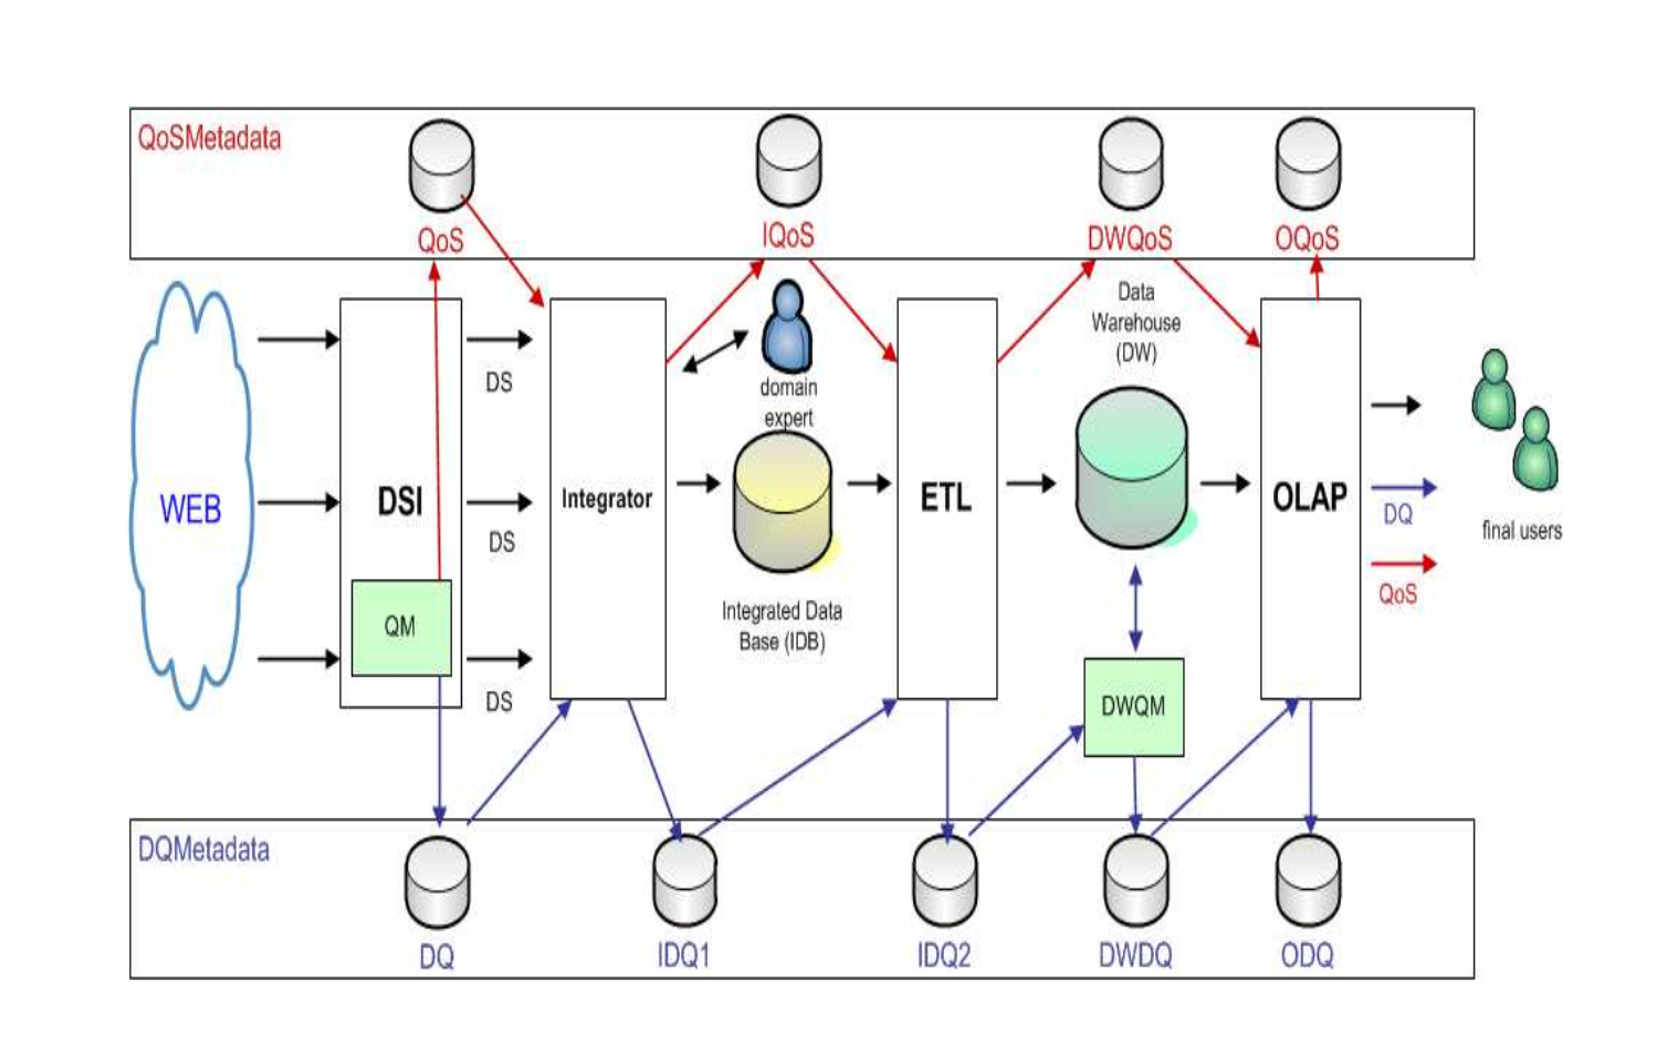
\includegraphics[scale=0.44]{arquitectura}
        \caption{Arquitectura del Data Warehouse}
        \label{dw_arq}
      \end{center}
    \end{figure}
   
    \begin{itemize}
      \item Lo primero que se puede notar en la Figura \ref{dw_arq} son las fuentes de datos, referenciadas en la primera propiedad presentada en la
      definición de Bill Inmon. Las distintas fuentes (posiblemente heterogéneas), son un factor a tenerse en cuenta cuando los
      datos son extraidos. Por ejemplo, la fuente de datos A pueden ser archivos planos de texto, la B archivos \textit{excel} y la C una base de datos 
      transaccional.
    
      \item Luego se observa el módulo \textbf{ETL}, acrónimo en inglés de \textbf{Extraction, Transformation and Loading} (Extracción, Transformación y Carga).
      En esta instancia es donde se aplican diversas técnicas para extraer la información obtenida de
      los diversos orígenes de datos. Luego, se realizan variadas transformaciones (dependiendo de la realidad en que se
      trabaja) para depurar e integrar los datos para cargarlos en un único repositorio central, con el fin de que en posteriores etapas se pueda obtener
      la información de forma sencilla y conociendo una única realidad. (se hace énfasis en esto último debido a que pueden darse situaciones de
      inconsistencia en los datos. Por ejemplo, 2 sectores de la empresa en cuestión informan valores distintos para la venta de un producto en el mismo
      período de tiempo).
    
      \item Seguido al módulo de ETL se observa el repositorio central donde se almacenan los datos depurados y listos para ser explotados utilizando
      diferentes técnicas. Si bien las que aparecen en la Figura \ref{dw_arq} son \textbf{OLAP} y \textbf{Data Mining}, existen muchas otras formas de 
      explotación, sobre las cuales no se entrará en detalles. Por ejemplo, construcción de reportes operativos, tableros de control, etc.
    \end{itemize}

    Todos y cada uno de los pasos, módulos y técnicas a los que se hicieron referencia al explicar la arquitectura de DW tienen como finalidad
    proveer de métodos y procedimientos sencillos con los cuales el usuario final pueda consultar la información almacenada, sin ningun conocimiento técnico y,
    además, pueda obtener la que le sea de utilidad para llevar a cabo un proceso de toma de decisiones simple y con mayor respaldo.
    
    
    \subsection{OLTP}
    
    Estas siglas componen el acrónimo de \textit{OnLine Transaction Processing} (Procesamiento de Transacciones En Línea). Es un tipo
    de procesamiento que facilita y administra aplicaciones transaccionales, usualmente para entrada y recuperación de datos y procesamiento de
    transacciones.
    Las aplicaciones OLTP tienen un alto rendimiento en la inserción o actualización intensiva de una base de datos. Estas aplicaciones son utilizadas
    simultáneamente por centenares de usuarios. Además, tienen como objetivos clave la disponibilidad, velocidad, concurrencia y recuperación.
    Por ejemplo, la aplicación que gestiona a determinado cajero automático de un banco, al tener que estar constantemente actualizando registros de una
    base de datos debido a las repititivas operaciones de depósitos o giros bancarios, es un claro ejemplo de una aplicación de procesamiento de
    transacciones comerciales.
    En definitiva, los sistemas OLTP son bases de datos orientadas al procesamiento de transacciones, entendiéndose una transacción como un proceso
    atómico (que debe ser validado con un commit, o invalidado con un rollback), y que puede involucrar operaciones de inserción, modificación y
    borrado de datos.\par
    
    Como se mencionó previamente, una de las formas de explotación de los datos almacenados en el DW es mediante OLAP, con lo cual creemos útil
    comparar los dos tipos de procesamiento. En la Figura \ref{oltp_vs_olap} se establece una comparación entre OLAP y OLTP,
    que considera los siguientes aspectos:
    
    \begin{figure}
      \begin{center}
        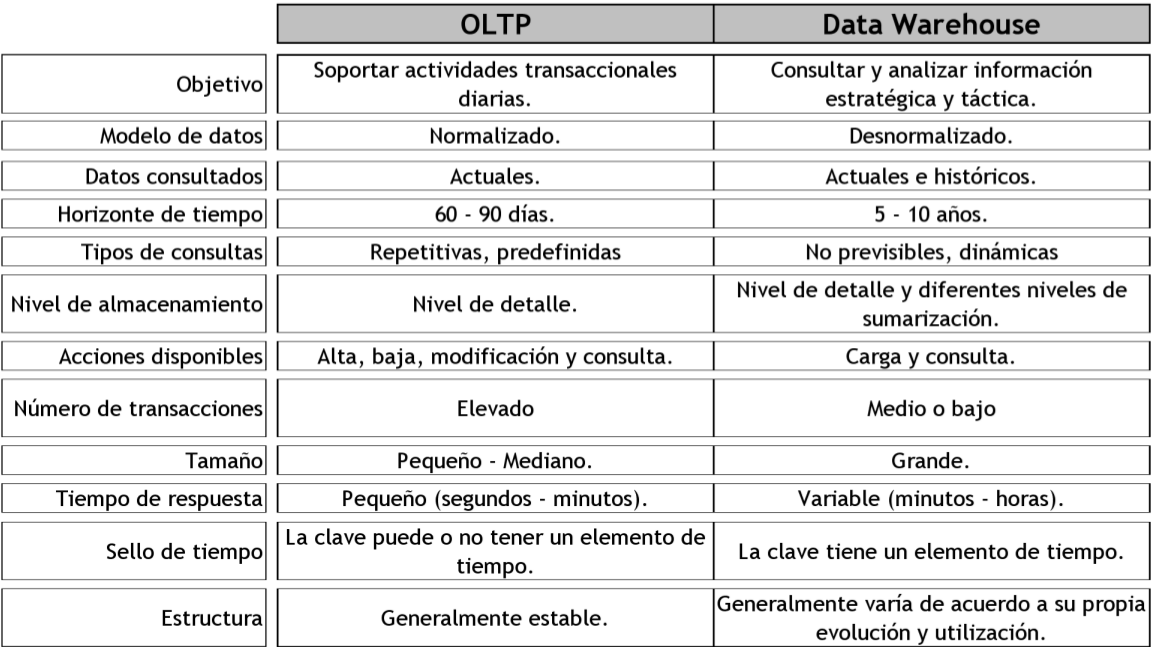
\includegraphics[scale=0.39]{OltpVSDW3}
        \caption{Cuadro comparativo entre el análisis OLTP y OLAP. \cite{hefestov2} Pag. 42.}
        \label{oltp_vs_olap}
      \end{center}
    \end{figure}
    
    
    \begin{itemize}
      \item \textbf{Objetivo:} 
        \begin{itemize}
          \item \textbf{Transaccional:} Diseñado para operaciones de negocio en tiempo real.
          \item \textbf{DW:} Orientado a las consultas y al análisis de los datos con el fin de asistir en la toma de decisiones. 
        \end{itemize}
      \item \textbf{Modelo de datos:}
        \begin{itemize}
          \item \textbf{Transaccional:} Normalizado; evita la redundancia de datos, con lo cual se minimiza el espacio de almacenamiento.
          \item \textbf{DW:} Desnormalizado, ya que esto favorece de rendimiento de las consultas, al reducir la cantidad de joins necesarios
          para obtener la información requerida (se sacrifica espacio en disco para obtener este beneficio).
        \end{itemize}
      \item \textbf{Datos consultados}
        \begin{itemize}
          \item \textbf{Transaccional:} Por la calidad de datos almacenados en las bases de datos transaccionales los datos requeridos son actuales.
          \item \textbf{DW:} Como se mencionó en las características de los DW, los datos almacenados son actuales e históricos, con lo cual se pueden
          consultar ambos tipos de datos.
        \end{itemize}
      \item \textbf{Horizonte de tiempo:}
        \begin{itemize}
          \item \textbf{Transaccional:} Tenemos un horizonte relativamente pequeño ya que las bases de datos transaccionales no tienen esta finalidad.
          \item \textbf{DW:} En este caso tenemos una amplia brecha de tiempo sobre la cual se guarda información ya que la misma es de mucho valor para
          la toma de decisiones.
        \end{itemize}
      \item \textbf{Tipo de consultas:}
        \begin{itemize}
          \item \textbf{Transaccional:} Las consultas disponibles pueden estar acotadas.
          \item \textbf{DW:} Tiene consultas impredecibles que acceden a muchas filas por tabla.
        \end{itemize}
      \item \textbf{Nivel de almacenamiento:}
        \begin{itemize}
          \item \textbf{Transaccional:} Se tiene los datos detallados al nivel definido al comienzo de la creación del esquema de la base de datos.
          \item \textbf{DW:} Al mismo nivel que en la base de datos transaccional y con distintos niveles de sumarización, con lo cual se logra un mayor
          rendimiento en el tiempo de respuesta.
        \end{itemize}
      \item \textbf{Acciones disponibles:}
        \begin{itemize}
          \item \textbf{Transaccional:} Alta, baja, modificación y consulta (insert, delete, update y select) son las acciones básicas.
          \item \textbf{DW:} Carga (Alta) y consulta, las bajas y modificaciones no se realizan debido a que queremos preservar la no volatilidad de los
          datos.
        \end{itemize}
      \item \textbf{Número de transacciones:}
        \begin{itemize}
          \item \textbf{Transaccional:} Soporta miles de usuarios de manera concurrente.
          \item \textbf{DW:} Soporta pocos usuarios simultáneamente, en relación a  OLTP.
        \end{itemize}
      \item \textbf{Tamaño:}
        \begin{itemize}
          \item \textbf{Transaccional:} Al almacenar sólo datos actuales, el tamaño de las bases de datos transaccionales suelen tener tamaños pequeños,
          en relación al DW.
          \item \textbf{DW:} Al contrario de las bases de datos transaccionales, al guardar datos históricos el tamaño de estas bases de datos suelen
          tornarse enormes.
        \end{itemize}
      \item \textbf{Tiempo de respuesta:}
        \begin{itemize}
          \item \textbf{Transaccional:} Está optimizada para un conjunto conocido de las transacciones, por lo general son la adición o la recuperación de
          una sola fila, a la vez, por tabla.
          \item \textbf{DW:} Debido al gran volumen de datos puede ocurrir que los tiempos de respuesta sean variables dependiendo de cada caso.
        \end{itemize}
      \item \textbf{Sello de tiempo:}
        \begin{itemize}
          \item \textbf{Transaccional:} Podría tener o no sello de tiempo, aunque para este tipo de bases de datos tener en cuenta el tiempo no es un
          factor decisivo.
          \item \textbf{DW:} Siempre tendremos una marca de tiempo ya que queremos preservar las característica de no volátil y variable en el tiempo.
        \end{itemize}
      \item \textbf{Estructura:}
        \begin{itemize}
          \item \textbf{Transaccional:} Debido a su utilización, la estructura definida en un comienzo no suele cambiar.
          \item \textbf{DW:} Por ser el mundo de los negocios un ambiente que está en constante evolución, se suele modificar la estructura para que capture
          estos cambios y la información siga aportando conocimiento de utilidad para la toma de decisiones.
        \end{itemize}
    \end{itemize}
    
    Debido a que los datos que son de utilidad (para el fin buscado) son los que contienen información histórica, y concluyendo que OLAP es el tipo
    de procesamiento que corresponde a estos datos (lo cual se deduce de la comparación anterior), a continuación se detallan algunas desventajas del
    procesamiento OLTP para clarificar aún más la diferencia entre ambos tipos de procesamiento:
    
    \begin{itemize}
      \item Gran rigidez a la hora de extraer datos, de manera que el usuario tiene que ceñirse a los informes predefinidos que se configuraron en el
      momento de la implementación, y que no siempre responden a sus dudas reales.
      \item Necesidad de conocimientos técnicos. Para la generación de nuevos informes o métricas suele resultar ineludible acudir al departamento técnico,
      solicitando una consulta adecuada para obetener los datos necesarios de la base de datos.
      \item Largos tiempos de respuesta, ya que las consultas complejas de datos suelen implicar la unión de tablas operacionales de gran tamaño, lo que se
      traduce en una incómoda espera que dificulta la fluidez del trabajo.
      \item Deterioro en el rendimiento del sistema de información. Cuando la base de datos consultada, para generar informes o ratios de negocio, es la
      misma que la que soporta el operativo de la empresa, el funcionamiento del sistema puede degradarse hasta afectar y paralizar a todos los usuarios
      conectados.
      \item Falta de integración que implica ``islas'' de datos. Muchas organizaciones disponen de múltiples sistemas de información, incorporados en
      momentos distintos, para resolver problemáticas diferentes. Sus bases de datos no suelen estar integradas, lo que implica la existencia de "islas"
      de información.
      \item Datos erróneos, obsoletos o incompletos. El tema de la calidad de los datos siempre es considerado como algo importante, pero esta labor nunca
      se lleva al extremo de garantizar la fiabilidad de la información aportada.
      \item Problemas para adecuar la información al cargo del usuario. No se trata de que todo el mundo tenga acceso a toda la información, sino de que
      tenga acceso a la información que necesita para que su trabajo sea lo más eficiente posible. Por ejemplo, en una organización compuesta por
      diferentes sectores A, B y C, una persona del sector A no debería poder acceder la información de los demás sectores ya que la misma probablemente
      no sea de relevancia para los fines que busca.
      \item Ausencia de información histórica. Los datos almacenados en los sistemas operacionales están diseñados para llevar la empresa al día, pero no
      permiten contrastar la situación actual con una situación retrospectiva de años atrás.
    \end{itemize}
    

    \subsection{Data Marts}
    
    \subsubsection{Definición}

    Los \textbf{Data Marts} (DM), son subconjuntos de datos de un \textit{Data Warehouse} para áreas específicas.
    Entre las características de un DM se destacan:
    
    \begin{itemize}
      \item Usuarios limitados
      \item Tiene un propósito específico
      \item Tiene una función de apoyo
    \end{itemize}
    
    Al hablar de un DM se dice que está destinado para un grupo de usuarios determinados ya que (por definición) está orientado a un área específica de la
    organización o empresa. De la misma observación puede entenderse que su propósito es ayudar en la toma de decisiones sobre el área que está enfocado.
    
    \subsubsection{Metodologías de diseño}
    
    \begin{itemize}
      \item \textbf{Top Down:} Como se puede apreciar en la Figura \ref{top_down}, el DW es cargado a través de procesos ETL y luego éste alimenta a los
      diferentes DM, cada uno de los cuales recibirá los datos que correspondan al tema o departamento que traten. Esta forma de implementación cuenta
      con la ventaja de no tener que incurrir en complicadas sincronizaciones de \textit{hechos}, pero requiere una gran inversión y más tiempo de
      construcción, que la arquitectura \textit{Bottom Up}.
      \item \textbf{Bottom Up:} En la Figura \ref{bottom_up} se ve claramente como los DM se cargan a través de procesos ETL, los cuales suministrarán la
      información adecuada a cada uno de ellos. En muchas ocasiones, los DM son implementados sin que exista el DW, ya que tienen sus mismas 
      características pero con la particularidad de que están enfocados en un tema específico, con lo cual el volumen de datos es mucho menor y, por ende,
      el manejo de los datos es más sencillo. Luego de haber sido creados y cargados todos los DM, se procede a su integración para obtener el
      respositorio central. La ventaja que trae aparejada este modelo es que cada DM se crea y pone en funcionamiento en un corto lapso de tiempo y se
      puede tener una pequeña solución a un costo no tan elevado. Luego que todos los DM estén puestos en marcha, se puede decidir si construir el DW o no.
      El mayor inconveniente está dado en tener que sincronizar los \textit{hechos} al momento de la consolidación del depósito central.
    \end{itemize}
    
    \begin{figure}
      \begin{center}
        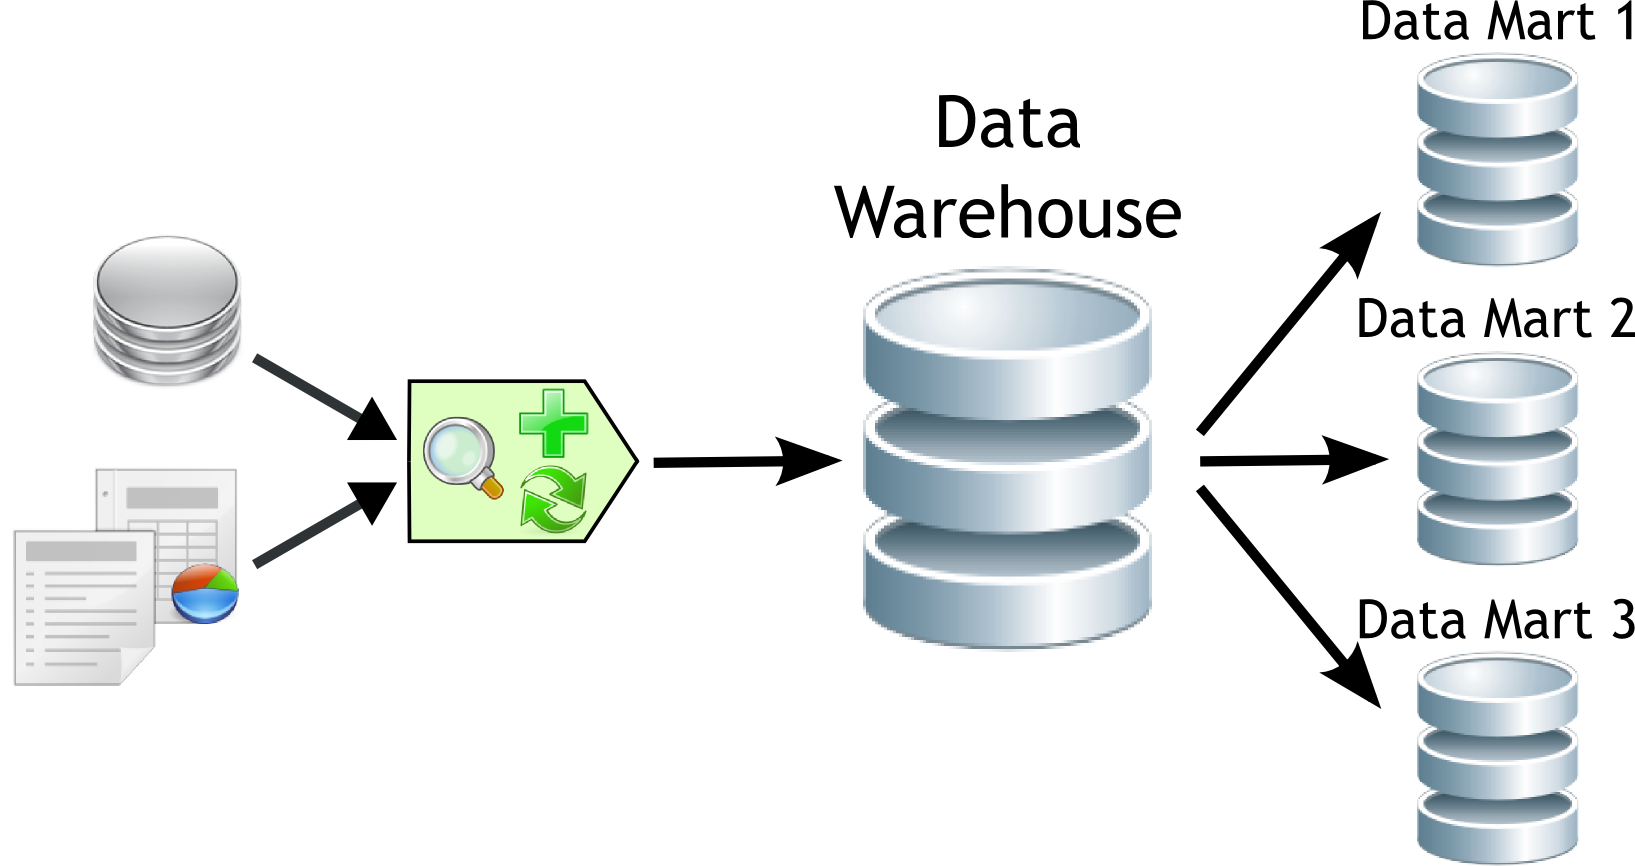
\includegraphics[scale=0.15]{Top-Down}
        \caption{Top Down} \cite{hefestov2} Pag. 74.
        \label{top_down}
      \end{center}
    \end{figure}
    
    \begin{figure}
      \begin{center}
        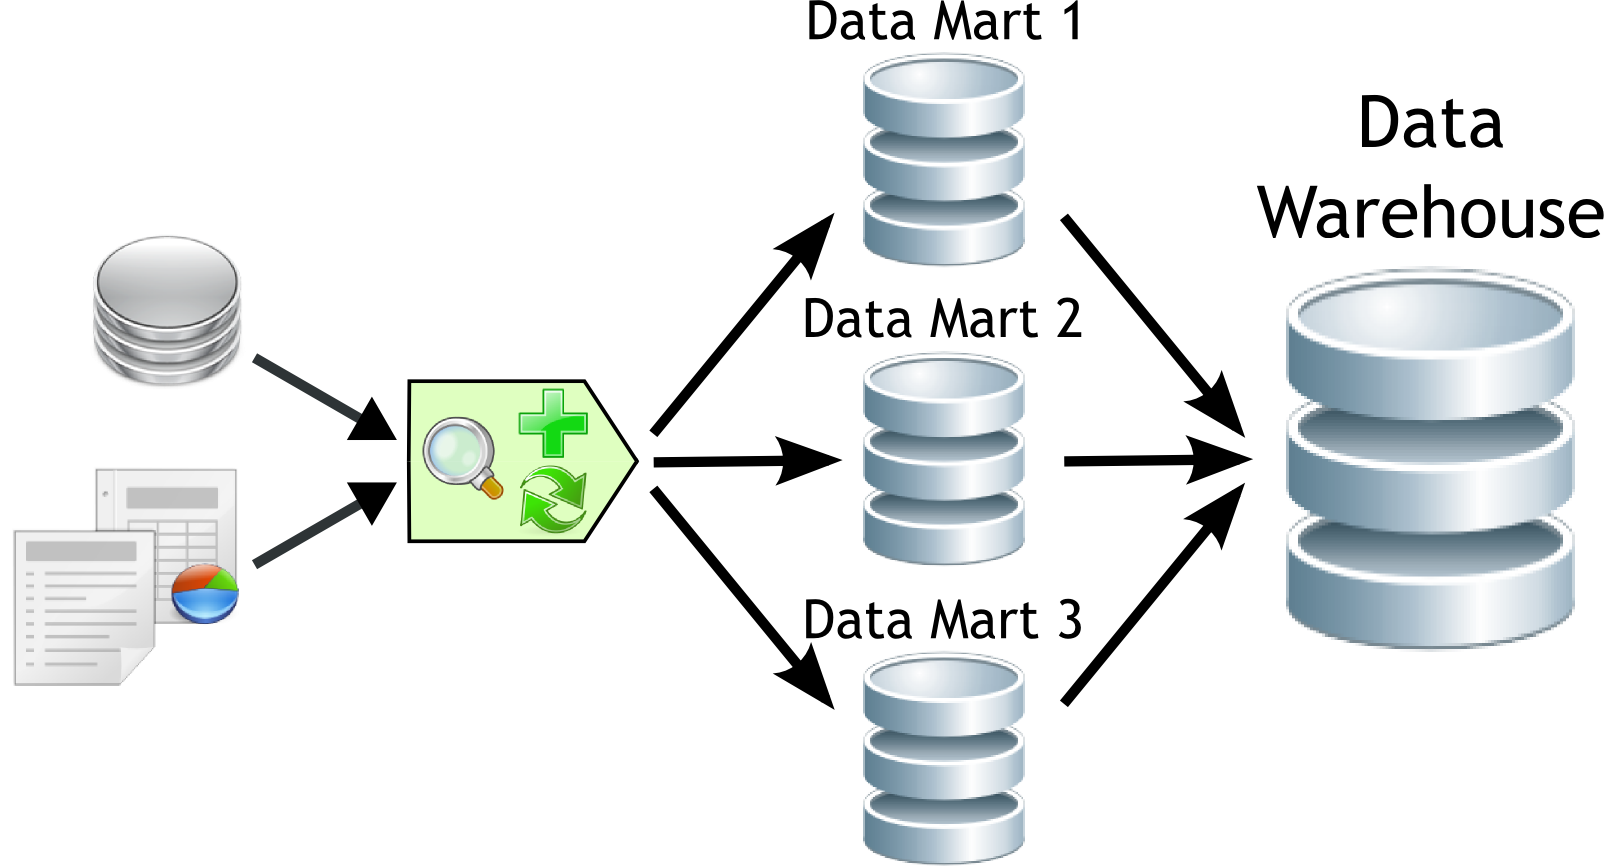
\includegraphics[scale=0.15]{Bottom-Up}
        \caption{Bottom Up} \cite{hefestov2} Pag. 74.
        \label{bottom_up}
      \end{center}
    \end{figure}
    
    
    \subsection{Modelo dimensional}
    
    El modelado dimensional es una técnica de diseño lógico de una base de datos, útil para el procesamiento OLAP, que tiene como ideas centrales el
    rendimiento y la comprendión, por parte de los usuarios, de los datos en forma sencilla.
    
    Los conceptos fundamentales del modelo dimensional son:
    
    \begin{itemize}
      \item \textbf{Hechos:} Son las medidas de negocios (o indicadores de negocios) que el usuario final quiere observar y sobre los cuales quiere tener
      conocimientos.
      \item \textbf{Dimensiones:} Éstas son las características que le dan contexto a lo que se quiere observar (hechos).
      Las dimensiones contienen datos cualitativos. Por ejemplo, si uno quiere observar el hecho total 
      vendido, las posibles dimensiones que le dan contexto a esta métrica son el tiempo, el negocio y la ciudad en que se ubica. Si bien cada dimensión hace
      referencia a un concepto específico aportando el contexto en el que se quiere observar el hecho, éste puede estructurarse con un orden jerárquico.
      Por ejemplo, si tenemos una dimensión país, dentro de la misma podríamos tener provincia y ciudad como dos niveles de granularidad. 
    \end{itemize}
    
    
    \subsection{Esquema dimensional}
    
    Se sabe que la relación entre todas las tablas de una base de datos se denomina esquema de base de datos. Para un cierto grupo de bases de datos, en las
    cuales se realizan consultas sobre datos históricos, generalmente se utilizan diseños llamados esquemas dimensionales. Un \textbf{esquema dimensional}
    separa físicamente las medidas que cuantifican el negocio (hechos) de los elementos que los describen (dimensiones). Estos tipos de diseños pueden ser de
    dos tipos:
    
    \begin{itemize}
      \item \textbf{Físico:} Generalmente los objetos que contiene son en realidad tablas de una base de datos.
      \item \textbf{Lógico:} Los hechos y las dimensiones se representan como entidades y atributos independientes a una base de datos y por lo tanto,
      se pueden transformar en un esquema dimensional físico para cualquier base de datos.
    \end{itemize}
    
    
    \subsection{Tipos de esquemas}
    
    \subsubsection{Esquema de estrella}
    
    Este tipo de esquemas tiene una tabla de hechos, rodeada de tablas de dimensiones. En la tabla de hechos habrá un campo por cada dimensión, que
    hace referencia a la clave primaria de la misma (a travez de la cual se podrá recuperar la información necesaria para cada hecho),
    y un campo por cada métrica que quiera ser evaluada. La combinación de los campos que referencian a las dimensiones forman, generalmente, la clave primaria de la
    tabla de hechos. Por otra parte, cada dimensión tendrá su campo clave y otros campos en los que se almacenan las correspondientes descripciones que son 
    de utilidad en el ambiente de negocios.
    
    Este esquema es ideal por su simplicidad y velocidad para ser usado en \textit{análisis multidimensionales}. Permite 
    acceder tanto a datos agregados como de detalle. El diseño de esquemas en estrella permite implementar la funcionalidad de una \textit{base de datos 
    multidimensional} utilizando una clásica base de datos relacional (más extendidas que las multidimensionales). Otra razón para utilizar los esquemas en 
    estrella es su simplicidad desde el punto de vista del usuario final. Las consultas son simples, ya que las condiciones y las uniones (Join) 
    necesarias sólo involucran a la tabla de hechos y a las de dimensiones, sin necesidad de que se encadenen uniones y condiciones a dos o más niveles como 
    es usual que ocurra en un esquema \textit{copo de nieve}.
    
    Consideremos el siguiente ejemplo: supóngase que se quiere realizar un análisis sobre el importe ganado por cliente, según el producto y en una fecha
    específica. Una posible representación utilizando un esquema estrella es el que se observa en la Figura \ref{star_sch}.
    
    Cuando se normaliza, se pretende eliminar la redundancia, la repetición de datos y que las claves sean independientes de
    las columnas, pero en este tipo de modelos se busca tener un formato desnormalizado para que al consultar información se requieran de pocos joins para
    poder obtenerla. En el ejemplo de la Figura \ref{star_sch} las tablas se encuentran desnormalizadas. Para apreciar la
    diferencia, en la Figura \ref{normalizado} muestra la tabla de productos normalizada.
    
    \begin{figure}
      \begin{center}
        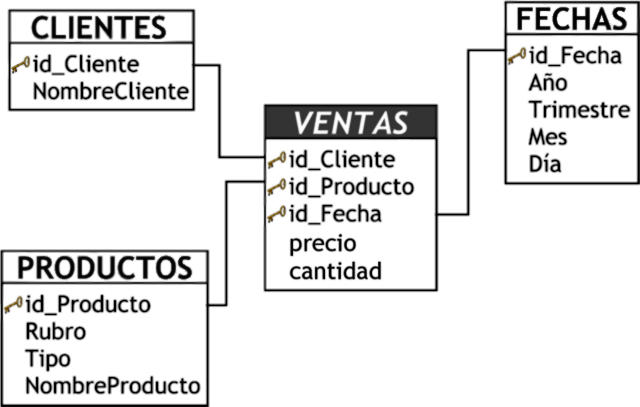
\includegraphics[scale=0.7]{esquema_estrella}
        \caption{Esquema de estrella. \cite{dim_models}}
        \label{star_sch}
      \end{center}
    \end{figure}
    
    \begin{figure}
      \begin{center}
        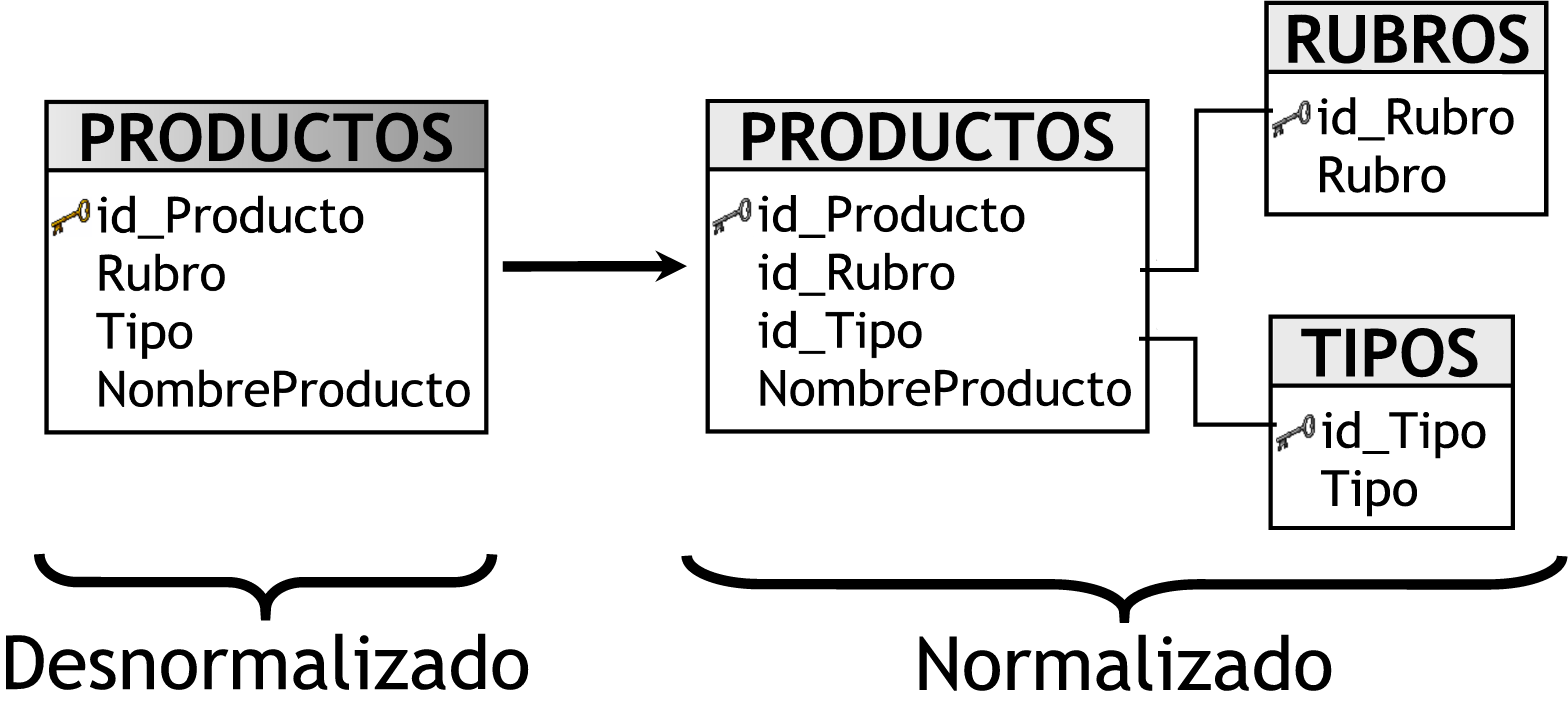
\includegraphics[scale=0.2]{normalizacion}
        \caption{Normalización de Productos. \cite{dim_models}}
        \label{normalizado}
      \end{center}
    \end{figure}
    
    
    \subsubsection{Esquema copo de nieve}
    
    Este es otro tipo de esquema, similar al esquema de estrella salvo por cierto detalle, las dimensiones pueden, a su vez, estar conectadas con otras 
    tablas de dimensiones. Es decir, habrá una tabla de hechos rodeada de tablas de dimensiones que nuevamente estén conectadas con otras tablas de 
    dimensiones, mediante una relación muchos a uno. Cada una de las dimensiones conectadas con otra dimensión representan un nivel jerárquico para la dimensión en 
    sí misma (por ejemplo, para la dimensión país, podríamos tener una tabla para país, otra para provincia y otra para ciudad). En el ejemplo de la Figura 
    \ref{snow_flk_sch} se ve claramente que una dimensión se implementa con más de una tabla. La razón de ésto es buscar la normalización de las tablas, con 
    lo cual se logra reducir espacio de almacenamiento al eliminar redundancia en los datos. Al tener una dimensión (la cual sería representada por una tabla 
    en la base de datos) representada por varias tablas, se facilita su mantenimiento.
    
    Este esquema tiene como finalidad reducir el espacio de almacenamiento, al eliminar la redundancia de datos, pero tiene como contrapartida
    peores rendimientos, en comparación al esquema estrella, al tener que mantener más tablas de dimensiones y más relaciones entre las tablas (Joins).
    
    \begin{figure}
      \begin{center}
        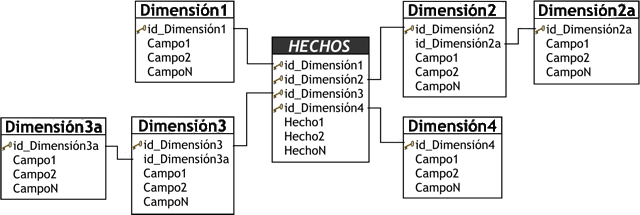
\includegraphics[scale=0.7]{copoNieve}
        \caption{Esquema copo de nieve. \cite{dim_models}}
        \label{snow_flk_sch}
      \end{center}
    \end{figure}
    
    
    \subsubsection{Esquema de constelación}
    
    Se compone de varios esquemas estrella y/o de copo de nieve. Pueden tener más de una tabla de hechos y compartir dimensiones, entre los hechos.
    La posibilidad de tener más de una tabla de hechos permite que una de ellas sea la principal y las demás contengan diversas sumarizaciones de información
    contenida en la principal.
    
    Este esquema es más complejo que los esquemas anteriores, debido a que contiene varias tablas de hechos. Si bien ésta es una solución flexible, puede 
    llegar a ser difícil de mantener. Puede ser de utilidad en algunos casos donde los hechos están asociados con un nivel de dimensión dada y otros hechos 
    con un nivel más bajo de la dimensión. Un ejemplo sencillo se plantea en la Figura \ref{const_sch} donde se pueden observar 2 tablas de hechos 
    compartiendo dimensiones.
    
    \begin{figure}
      \begin{center}
        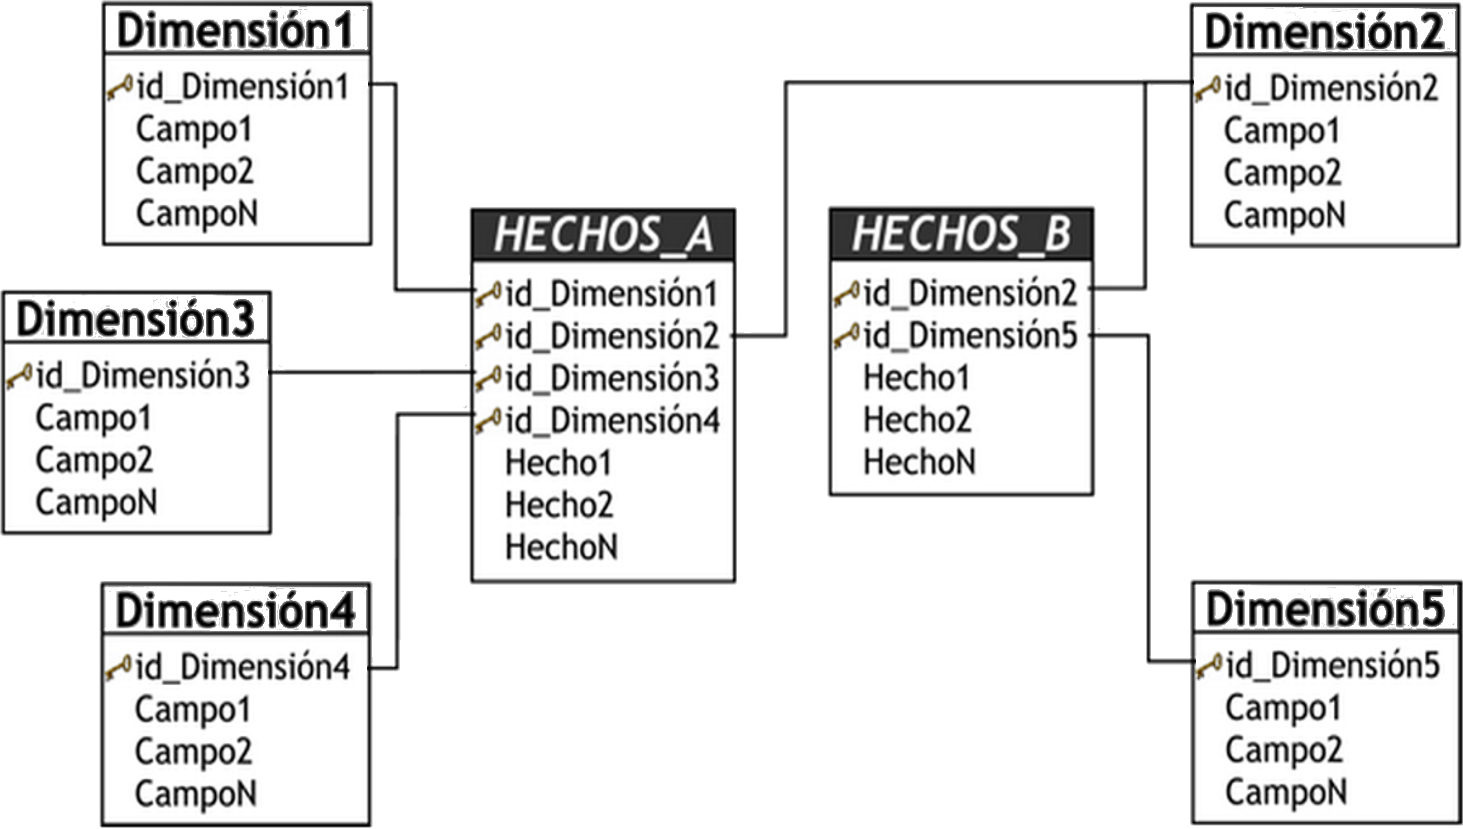
\includegraphics[scale=0.25]{esquema_constelacion}
        \caption{Esquema de constelación. \cite{dim_models}}
        \label{const_sch}
      \end{center}
    \end{figure}
    
    
    \subsection{Bases de datos temporales}
    
    Una \textbf{base de datos temporal} es una base de datos que trata con especial énfasis aspectos temporales, teniendo un modelo de datos temporal y una versión
    temporal del lenguaje de consulta estructurado.
    
    Los datos almacenados en una base de datos temporal tienen un asociado un período de tiempo que expresa su validez. Las bases de datos convencionales
    consideran que los datos almacenados en ella son válidos, sin importar el tiempo, ya que no mantienen un registro de los estados pasados o futuros de
    la base de datos. En cambio, las bases de datos temporales hacen posible almacenar diferentes estados de la base de datos. Por ésto, podemos
    considerar al DW como una base de datos temporal.
    
    
    \subsection{Dimensión de tiempo}
    
    En un DW, la creación y el mantenimiento de una tabla de dimensión \textbf{Tiempo} es obligatoria, y la definición de granularidad y estructuración de la misma 
    depende de la dinámica del negocio que se esté analizando. Toda la información del DW, como ya se ha explicado, posee su propio sello de 
    tiempo, el cual determina la ocurrencia de un hecho específico, representando de esta manera, diferentes versiones de una misma situación.Al momento de 
    implementar la dimensión como una tabla en una base de datos se debe tener especial cuidado con el campo clave que se elige ya que esto puede influir 
    mucho en el espacio que se ocupará en disco y los tiempos de respuesta.\par
    
    A continuación se detallan las representaciones más frecuentes del tipo de dato utilizado para la clave:
    
    \begin{itemize}
      \item \textbf{Date:} Si se usa Date como tipo para  el campo clave, costaría mucho espacio en comparación con un entero y los tiempos de respuesta se
      relentizarán ya que para los motores de consulta es más costosa la comparación con este tipo de campos que con uno entero.
      \item \textbf{Entero:}
      \begin{itemize}
        \item Se puede utilizar un campo autoincremental, el cual tiene la siguiente forma: 1, 2, 3, \dots con lo cual el costo de almacenamiento en disco
        se reduciría considerablemente y los tiempos de respuesta bajan ya que la comparación entre enteros no es algo costoso. Sin embargo, con esta representación se
        torna confuso saber con qué fecha se está trabajando.
        \item Una mejor opción es utilizar un campo de la forma yyyyMMdd, por ejemplo 20150315, ya que se obtienen los mismos benefícios que los planteados
        en el item anterior a lo que se suma una mejor comprensión a la hora de visualizar los registros.
      \end{itemize}
    \end{itemize}
    
    
    \section{OnLine Analytical Processing}
    
    Más conocido por su acrónimo OLAP (Procesamiento Analítico En Línea), es una solución utilizada en el campo de la inteligencia de negocios, cuyo 
    objetivo es permitir la consulta de grandes cantidades de datos de forma eficiente y sencilla. Utiliza estructuras multidimensionales (cubos OLAP) que 
    contienen datos resumidos de grandes bases de datos.
    
    Como se explico anteriormente, en una base de datos transaccional, normalmente se estructuran las tablas con un modelo normalizado, lo cual favorece a
    la explotación OLTP, en cambio, las bases de datos configuradas para OLAP utilizan un modelo de datos multidimensional, lo que permite consultas 
    analíticas complejas, con tiempos de ejecución más reducidos, que su contrapartida OLTP.

    Las técnicas OLAP, e incluso OLTP fueron iniciadas por E.F. Codd \footnote{El Dr. Codd fue un investigador de base de datos, muy conocido a partir de la
    década de 1960. Es considerado el inventor del modelo de base de datos relacional en 1969.}, considerado el padre de las bases de datos
    relacionales. Las aplicaciones típicas de OLAP se circunscriben en los siguientes ámbitos: informes de negocio de ventas, marketing, informes de gestión,
    gestión del rendimiento empresarial (BMP), presupuestos y previsiones, informes financieros, etc.
    
    
    \subsection{Reglas de Codd}
    
    En 1993, E.F. Codd \& Associates publicó un informe, encargado por Arbor Software (ahora Hyperion Solutions), titulado "Providing OLAP to User-Analysts:
    An IT Mandate".
    En un comienzo Codd definió 12 reglas con el fin de evitar que la visión que él tenía sobre las bases de datos relacionales se perdiera, y con el correr
    de los años se extendieron a 18 \footnote{Se pueden observar en \cite{nagabhushana} Pag. 205}. A continuación se detallan las reglas más importantes 
    para los autores:
    
    \begin{itemize}
      \item \textbf{Visión multidimensional:} Las bases de datos OLAP siguen el modelo dimensional. Por lotanto, OLAP debe ofrecer al usuario final
      una visión de todas las dimensiones del modelo. Provee la base para el procesamiento analítico mediante un acceso flexible y simple a los datos de la 
      organización o empresa.
      \item \textbf{Manipulación intuitiva de los datos:} Lo que se intenta remarcar con esta regla es que tiene que la navegación de los datos debe ser
      sencilla, para lo cual, la mayoría de las aplicaciones ofrecen el doble click o el drag and drop para acceder a los datos.
      \item \textbf{Accesibilidad:} Esto está relacionado con el item anterior, salvo que de una forma un poco más abstracta. Lo que plantea es que se
      considera a las aplicaciones OLAP como el middleware (capa intermedia) entre las distintas fuentes de información y el usuario final.
      \item \textbf{Soporte de multi-usuario:} La aplicación OLAP debe soportar accesos concurrentes, lo que conlleva a mantener la integridad y seguridad
      de la misma.
      \item \textbf{Información separada del origen de datos:} Esto hace referencia a lo explicado en la arquitectura de DW, ya que se almacena toda la
      información que se va a analizar en el repositorio central, el cual se encuentra separado las fuentes de datos.
      \item \textbf{Flexibilidad ante valores nulos:} Esto punto se refiere a que ante la presencia de valores nulos (posiblemente por no estar informados)
      se diferencien de los valores en 0, lo cual influye en gran medida en los cálculos matemáticos (por ejemplo, podrían no ser considerados en el cálculos
      de promedios). Por otro lado, se debe ofrecer la posibilidad de excluir estos valores para que solamente se visualicen los valores realmente
      importantes.
      \item \textbf{Rendimiento uniforme:} Sin importar la cantidad de dimensiones ni el tamaño que tenga la base de datos, el rendimiento no debe verse
      afectado significativamente.
      \item \textbf{Dimensiones y niveles de agregación ilimitados:} Técnicamente ningún producto puede satisfacer esta regla ya que no se disponen de
      recursos ilimitados. De todos modos, en general, la cantidad de dimensiones y los niveles de agregación varían dependiendo del negocio u organización.
      Son pocas las aplicaciones que necesitan más de 10 dimensiones y jerarquías con más de 6 niveles. Codd sugiere un máximo de entre 15 y 20 dimensiones.
      En cualquier caso, se debe tener en cuenta que la herramienta que se compre tiene sus limitaciones.
    \end{itemize}
    
    
    \subsection{FASMI}
    
    Las reglas de Codd fueron inadecuadas para detectar ``productos OLAP'', por lo que los investigadores se vieron obligados a crear su propia
    definición. La definición debía que ser simple, memorable e independiente del producto, lo que resultó en la prueba FASMI \footnote{Explicada en
    \cite{nagabhushana} Pág. 204.}, Fast Analysis of Shared Multidimentional Information (Análisis Rápido de Información 
    Multidimensional Compartida). Cada componente de esta sigla tiene un significado particular y son explicadas a continuación:
    
    \begin{itemize}
      \item \textbf{Rápido:} Los vendedores recurren a una amplia variedad de técnicas para lograr este objetivo, incluyendo formas especializadas de
      almacenamiento de datos, extensos cálculos previos y requisitos de hardware específicos, pero se cree que ningún producto esté aún completamente
      optimizado en cuanto al tiempo de respuesta, por lo que éste punto se encuentra en un estado de desarrollo.
      El OLAP Survey \footnote{Encuesta a través de los principales productos OLAP, duranter 5 años (2001 a 2005).} encontró
      que la lentitud de las respuestas a las consultas, son el problema técnico más frecuente en los productos OLAP, claramente muchas implementaciones
      no superan esta prueba.
      \item \textbf{Análisis:} Los productos deben permitir al usuario definir nuevos cálculos \textit{ad hoc} como parte del análisis e informar los datos de la
      forma en que el usuario lo desee, sin requerir conocimientos técnicos. Ésto podría incluir características como el análisis de series de tiempo,las
      asignaciones de costos, la conversión de moneda, búsqueda de objetivos, los cambios estructurales multidimensionales ad hoc, y otras funciones que
      dependen de la aplicación.
      \item \textbf{Información:} Se está midiendo la capacidad de los distintos productos en términos de la cantidad de datos de entrada que puede manejar,
      no de cuántos gigabytes utilizan para almacenarlo.
      \item \textbf{Multidimensional:} El tipo de información con que se trata concuerda con el tipo de modelos dimensionales nombrados en las anteriores
      secciones, con lo cual la estructura multidimensional subyacente queda al descubierto.
      \item \textbf{Compartida:} No todas las aplicaciones permiten la escritura de datos, pero si lo hace, el sistema debe ser capaz de manejar múltiples
      actualizaciones de manera oportuna.
    \end{itemize}
     
    
    \subsection{Jerarquías}
    
    Las dimensiones en general, tienen distintos niveles \footnote{Se detalla en \cite{olap_solutions} Pag. 94.}, los cuales representan las
    múltiples granularidades de la dimensión (menor o mayor nivel de detalle). Estos niveles forman parte de una jerarquía. El ejemplo más simple de
    jerarquía es el de la dimensión de tiempo, la cual puede ser: \textbf{Año > Mes > Día}. Tanto en la dimensión de
    tiempo como en cualquier otra existe la posibilidad de definir distintas jerarquías. Dos ejemplos sencillos se ilustran en la Figura
    \ref{jerarquias}.
    
    \begin{figure}
      \begin{center}
        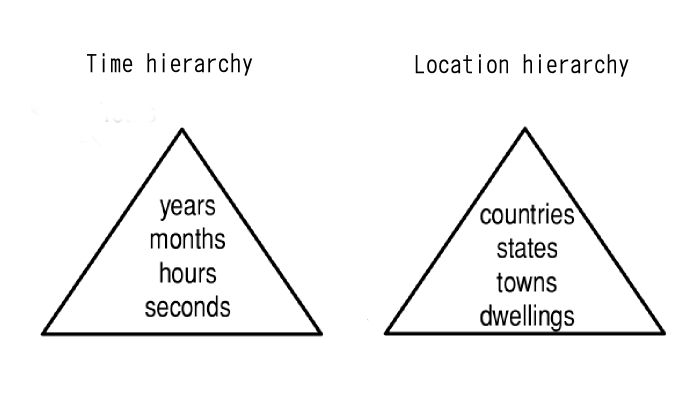
\includegraphics[scale=0.5]{jerarquias}
        \caption{Jerarquías de \textit{Tiempo} y \textit{Ubicación}. \cite{olap_solutions} Pag. 94.}
        \label{jerarquias}
      \end{center}
    \end{figure}
    
    
    \subsection{Agregaciones}
    
    El modelo dimensional permite optimizar el rendimiento de las consulta mediante la creación de tablas agregadas. El número de posibles agregaciones se
    determina por las combinaciones posibles de las distintas granularidades de cada dimensión. Dado que sería muy costoso construir todas las agregaciones 
    posibles, es una buena idea elegir un subconjunto de tablas sobre las cuales hacer agregaciones. La mejor manera de elegir este subconjunto y decidir qué 
    agregaciones construir, es monitorear las consultas, y diseñar las agregaciones que coincidan con los patrones de consulta.\par
    
    En las Figura \ref{sch_orig1}, se puede apreciar el esquema base sin agregaciones, y en la Figura \ref{sch_agg1} vemos el esquema
    donde los campos tienen un determinado nivel de agregación.
    
    \begin{figure}
      \begin{center}
        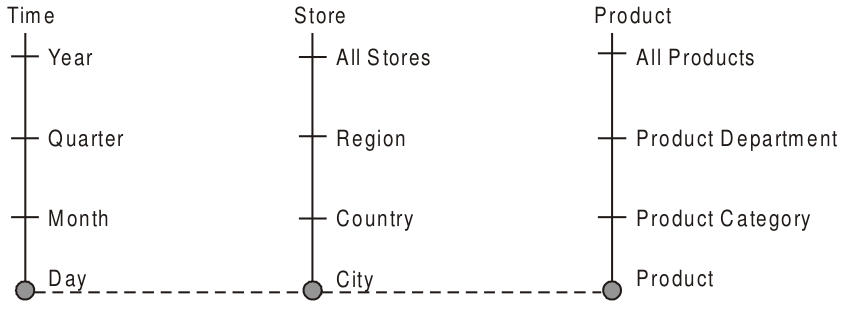
\includegraphics[scale=0.3]{esq_orig1}
        \caption{\textbf{Esquema de nivel base}, contiene los datos en el nivel más detallado. \cite{nagabhushana} Pag. 172.}
        \label{sch_orig1}
      \end{center}
    \end{figure}
    
    \begin{figure}
      \begin{center}
        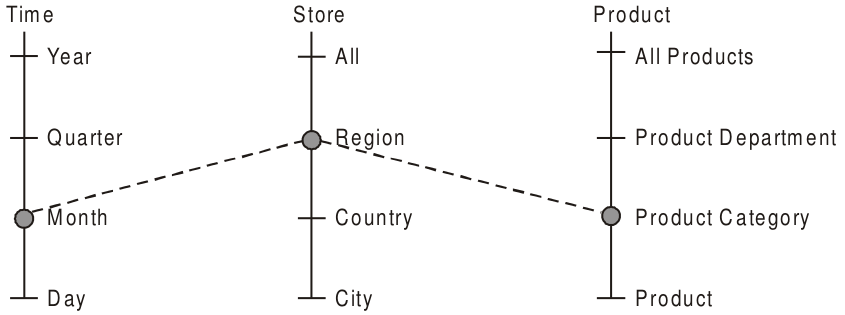
\includegraphics[scale=0.3]{esq_agg1}
        \caption{\textbf{Esquema agregado}, tiene datos en los niveles más alto de las jerarquías. \cite{nagabhushana} Pag. 172.}
        \label{sch_agg1}
      \end{center}
    \end{figure}
    
    
    Los esquemas agregados proporcionan mejoras en el rendimiento, ya que la cantidad de registros se reduce consirablemente respecto al esquema base. El
    uso más común de los agregados es tomar una dimensión determinada y cambiar su granularidad. Al hacer ésto, la tabla de hechos debe ser parcialmente
    resumida para adaptarse a la nueva dimensión. Se crean así, nuevas tablas de dimensión y de hechos, que encajan en el nuevo nivel de granularidad deseado.
    
    En la Figura \ref{sch_orig2} vemos, a modo ejemplo, un esquema copo de nieve con una tabla de hechos y 3 dimensiones.\footnote{Notar que la
    dimensión \textit{Product} está normalizada.} Además, en la Figura \ref{sch_agg2} se puede observar una tabla agregada donde se combinan las tablas de la
    Figura \ref{sch_orig2} de la siguiente forma:
    
    \begin{itemize}
      \item La dimensión de \textit{Time} ``colapsó'' en la tabla de agregación, donde se omitieron los campos \textit{month} y \textit{day}.
      \item Las dos tablas que conforman a la dimensión \textit{Product} colapsaron en la tabla de agregación.
      \item La dimensión \textit{Customer} se dejó de tener en cuenta, en la tabla agregada.
      \item Para cada métrica en la tabla de hechos (\textit{units}, \textit{dollars}) hay una o más métricas en la tabla de 
      agregación (\textit{sum units, min units, max units, sum dollars}).
      \item También se genera una nueva métrica (\textit{row count}) que representa el conteo de las filas.
    \end{itemize}
    
    \begin{figure}
      \begin{center}
        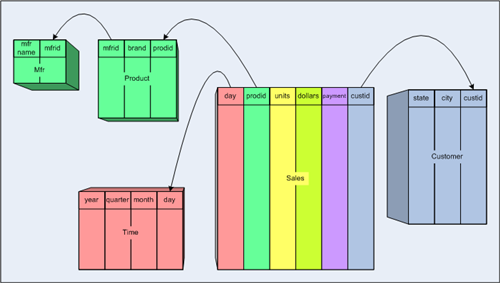
\includegraphics[scale=0.8]{esq_orig2}
        \caption{Esquema original. \cite{agg_tables}}
        \label{sch_orig2}
      \end{center}
    \end{figure}
    
    \begin{figure}
      \begin{center}
        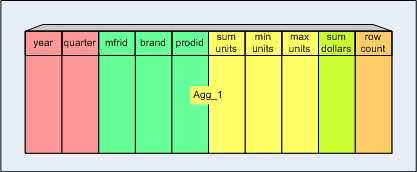
\includegraphics[scale=0.8]{esq_agg2}
        \caption{Esquema agregado. \cite{agg_tables}}
        \label{sch_agg2}
      \end{center}
    \end{figure}
    
    Tener datos agregados en el modelo dimensional hace al entorno más complejo. Para que esta complejidad sea transparente al usuario, se utiliza
    una funcionalidad conocida como \textit{navegación de agregados}, la cual es implementada por el motor OLAP, que permite consultar las
    tablas dimensionales y de hechos, con el nivel de granularidad correcto.
    
    
    \subsection{Hipercubo de datos}
    
    En la construcción de cubos OLAP, las tablas de dimensiones son elementos que contienen atributos (o campos) que se utilizan para restringir y agrupar
    los datos almacenados en una tabla de hechos cuando se realizan consultas sobre dichos datos en un DW o DM. Estos datos sobre dimensiones son parámetros
    de los que dependen otros datos que serán objeto de estudio y análisis y que están contenidos en la tabla de hechos. Las tablas de dimensiones ayudan a
    realizar ese estudio/análisis aportando información sobre los datos de la tabla de hechos, por lo que puede decirse que en un cubo OLAP, la tabla de
    hechos contiene los datos de interés y las tablas de dimensiones contienen metadatos sobre dichos hechos.

    El camino hacia la comprensión de los hipercubos no pasa a través de la longitud, ancho y alto de un cubo físico, el cubo es una metáfora visual. Hay
    límites naturales con respecto a lo que se puede hacer en una pantalla de dos dimensiones. Esta limitación ha hecho pensar largo y tendido a los
    desarrolladores de software acerca de la forma óptima de representar la información con más de dos dimensiones en una pantalla de computadora plana a
    efectos de la visualización y manipulación.
    
    Para concretizar la idea de visualización de un cubo se utilizará el conjunto de datos de la Figura \ref{tab_cube} donde se pueden observar una basta cantidad de
    métricas \textbf{(Sales, Direct Costs, Indirect Costs, Total Costs y Margin)} y una única dimensión (Month) que representa la dimensión de tiempo. Es
    importante hacer la aclaración de que el conjunto de métricas se considera como una dimensión en sí misma, con lo cual hay 2 dimensiones en el esquema de
    los datos del ejemplo planteado. Al agregarse una tercer dimensión (Products) se obtiene un cubo en el cual cada celda contiene el valor para un un mes,
    un producto y una métrica determinada, como se puede apreciar en el gráfico de la Figura \ref{cube_2}.
    
    \begin{figure}
      \begin{center}
        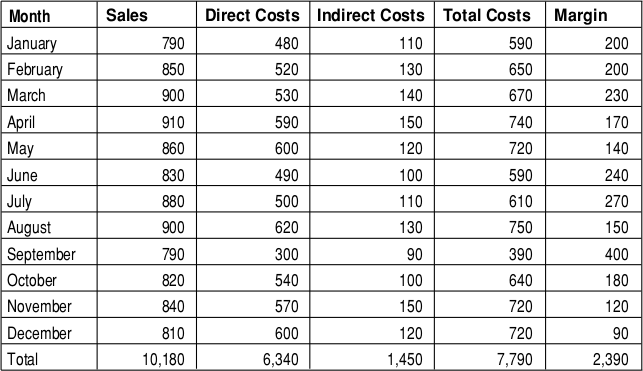
\includegraphics[scale=0.5]{cube_1}
        \caption{Conjunto de datos} \cite{olap_solutions} Pag. 48.
        \label{tab_cube}
      \end{center}
    \end{figure}
    
    \begin{figure}
      \begin{center}
        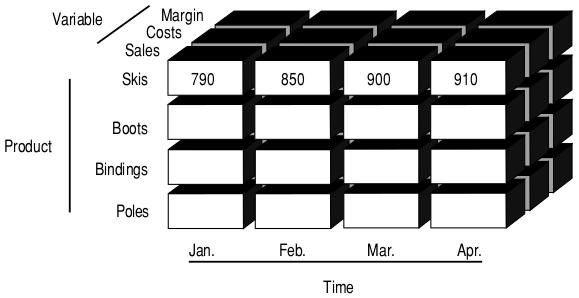
\includegraphics[scale=0.6]{cube_2}
        \caption{Cubo con 3 dimensiones: \textbf{Variable, Time, Product}} \cite{olap_solutions} Pag. 49.
        \label{cube_2}
      \end{center}
    \end{figure}
    
    
    Una de las opciones para poder representar este cubo tridimensional acotado por las restricciones de una pantalla de dos dimensiones es tomar una
    "rebanada" del mismo. Ésto consiste en fijar una de las dimensiones (por ejemplo, la de Producto) a un valor determinado, con lo cual se obtendrá una
    tabla cuyas celdas contendran información para los cruces de los valores de las otras 2 dimensiones respecto al producto seleccionado. En la Figura
    \ref{cube_3} se puede observar la visualización del cubo de la Figura \ref{cube_2} habiendo seleccionado el producto shoes. Al resultado obtenido se
    lo llama página o rebanada.\par 
    
    \begin{figure}
      \begin{center}
        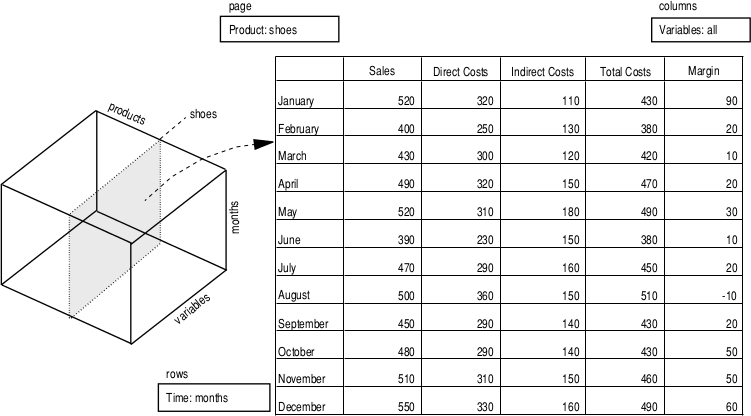
\includegraphics[scale=0.5]{cube_3}
        \caption{\textbf{Visualización de cubo:} "rebanada" del cubo seleccionando un valor específico de la dimensión product} \cite{olap_solutions} Pag. 51.
        \label{cube_3}
      \end{center}
    \end{figure}
    
    
    Al añadir una cuarta dimensión al cubo, utilizando la técnica que se planteó hasta el momento, no será posible obtener una visualización del mismo en una
    pantalla de dos dimensiones. A partir de la anterior limitación, surge la necesidad de plantear una nueva estructura que permita la representación de los
    datos si que se restrinja la cantidad de dimensiones a utilizar, a éstas se las llama estructuras de tipo multidimensional (en inglés, Multidimensional Type
    Structures) o MTS. Cada dimensión se representa por una línea y cada miembro dentro de la dimensión será representado por un intervalo o segmento. Para
    clarificar la idea, se representará el ejemplo presentado en la Figura \ref{cube_2} utilizando estas estructuras. En la Figura \ref{cube_4} se puede observar
    la completa representación.
    
    \begin{figure}
      \begin{center}
        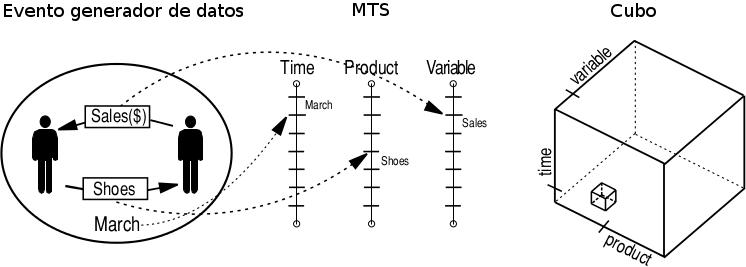
\includegraphics[scale=0.6]{cube_4}
        \caption{Ejemplo de representación utilizando \textbf{MTS}} \cite{olap_solutions} Pag. 55.
        \label{cube_4}
      \end{center}
    \end{figure}
    
    
    \subsection{Hipercubo en pantalla}
    
    Para poder lograr que los datos se visualicen de forma correcta por pantalla se deberá mapear las múltiples dimensiones lógicas en las dos dimensiones físicas
    que utiliza el monitor, para ésto se debe comenzar por transformar dos dimensiones en una, lo cual se logra anidando una dimensión dentro de la otra. En las
    Figuras \ref{cube_5} y \ref{cube_6} se muestran 2 formas en las que se puede llevar a cabo el procedimiento utilizando las dimensiones de las variables y los
    productos. En la Figura \ref{cube_7} se puede observar un escenario más elaborado en el que se agregan las dimensiones de Tiendas (Stores), Clientes
    (Customers) y Escenarios (Scenarios), donde se pueden apreciar múltiples anidamientos para obtener como resultado final una representación bidimensional de
    las 6 dimensiones.
    
    \begin{figure}
      \begin{center}
        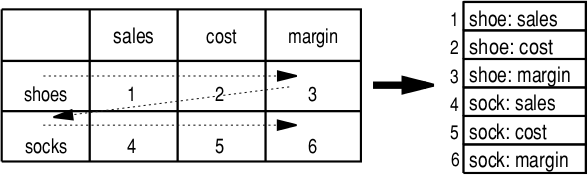
\includegraphics[scale=0.4]{cube_5}
        \caption{Transformación de 2 dimensiones a 1: Variables anidadas en Productos} \cite{olap_solutions} Pag. 58.
        \label{cube_5}
      \end{center}
    \end{figure}
    
    \begin{figure}
      \begin{center}
        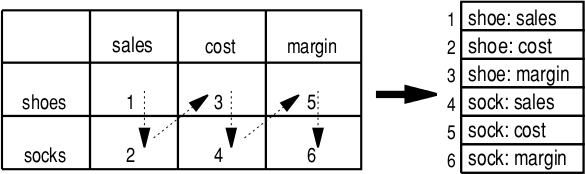
\includegraphics[scale=0.4]{cube_6}
        \caption{Transformación de 2 dimensiones a 1: Productos anidados en Variables} \cite{olap_solutions} Pag. 58.
        \label{cube_6}
      \end{center}
    \end{figure}
    
    \begin{figure}
      \begin{center}
        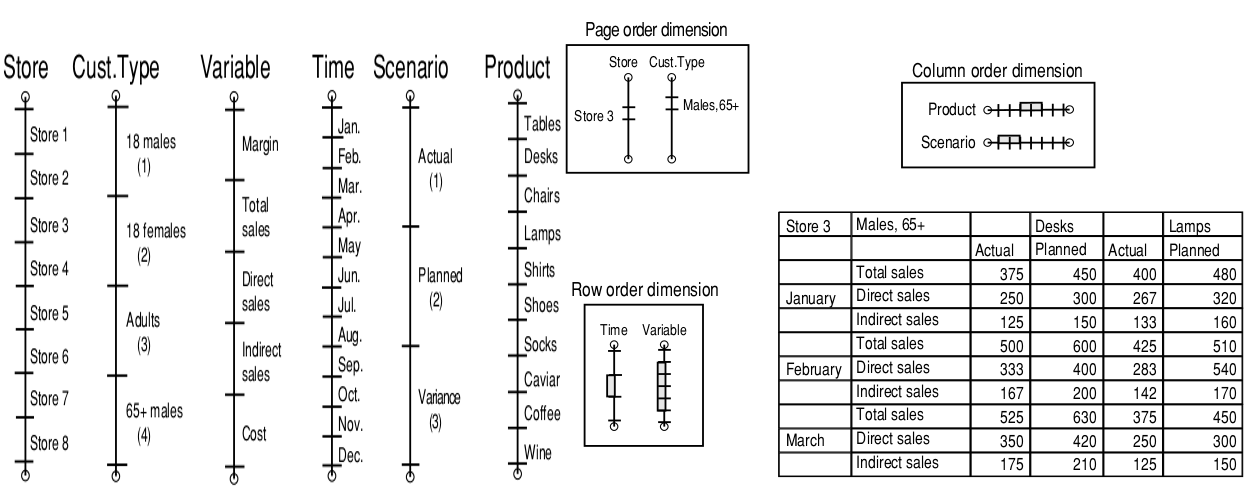
\includegraphics[scale=0.4]{cube_7}
        \caption{Anidamiento de 6 dimensiones} \cite{olap_solutions} Pag. 60.
        \label{cube_7}
      \end{center}
    \end{figure}
    
    
    La capacidad de cambiar fácilmente las vistas de los datos, mediante la reconfiguración de cómo se muestran las dimensiones, es uno de los grandes beneficios
    que proveen los sistemas multidimensionales, lo que es primordial en el momento en que los usuarios finales navegan en busca de información. La gran
    flexibilidad provista para alterar la estructuración de los datos se debe en gran medida la las MTS.\par
    
    \vspace{0.2in}
    Al analizar datos multidimensionales es de mucha utilidad tener en consideración las siguientes reglas básicas para poder comprender más a fondo el panorama
    de los mismos y, así, lograr mejores resultados:
    
    \begin{itemize}
      \item Tratar de utilizar páginas, lo cual permite visualizar la información de mayor relevancia en la pantalla.
      \item Cuando se necesite anidar múltiples dimensiones a través de las filas y columnas, generalmente, es mejor anidar más dimensiones en las columnas que
      a través de filas, ya que las pantallas suelen tener más espacio horizontal que vertical.
      \item Antes de decidir cómo mostrar la información en la pantalla, resolver los siguientes interrogantes:
        \begin{enumerate}
          \item ¿Qué se quiere observar?
          \item ¿Qué se intenta comparar?
        \end{enumerate}
    \end{itemize}
    
    
    \subsection{Operaciones}
    
    A continuación se detallan las operaciones que los autores consideran como las más importantes dentro del ámbito OLAP, y junto con las mismas se grafican
    ejemplos para lograr una mejor comprensión del lector y un mayor entendimiento:
    
    \begin{itemize}
      \item \textbf{Slice:} En esta operación se selecciona un valor particular de una de las dimensiones del cubo, buscando con ésto obtener una "rebanada" del
      mismo.
      \item \textbf{Dice:} Seleccionar valores específicos de 2 o más dimensiones de las cuales se visualizan y así obtener un subcubo del cubo original.
      \item \textbf{Drill Down:} Esta operación busca ofrecer más detalle respecto a la información que actualmente se puede visualizar. Lo antedicho puede
      lograrse de 2 formas, bajar un nivel en la jerarquía de una dimensión en particular o agregar una dimensión para sumar aún más información sobre el contexto.
      \item \textbf{Drill up:} En contraposición con la anterior operación, lo que se intenta lograr es visualizar menos información, lo cual puede realizarse
      subiendo un nivel en la jerarquía de una dimensión o eliminando alguna de las dimensiones. De esta forma información con un nivel de abstracción más alto.
      \item \textbf{Pivot:} Aplicando esta operación se ofrece al usuario una presentación alternativa de la información rotando los ejes de datos.
    \end{itemize}
    
    \begin{figure}
      \begin{center}
        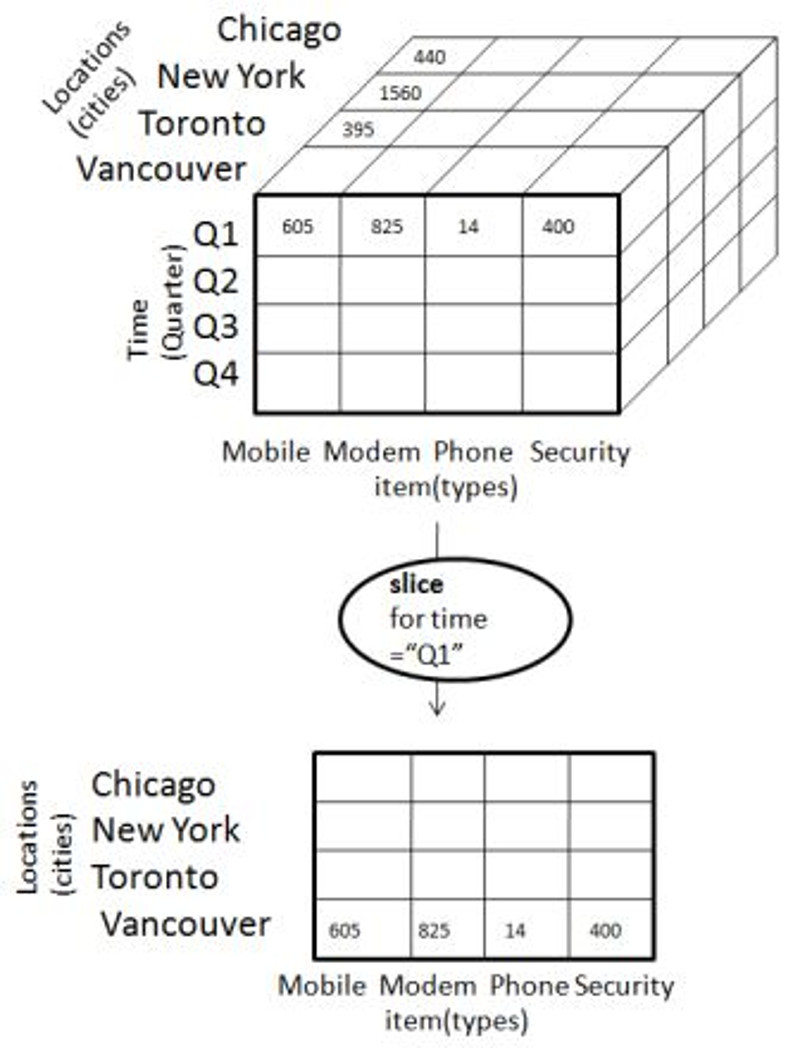
\includegraphics[scale=0.4]{slice}
        \caption{Operación Slice} \cite{operaciones}
        \label{slice}
      \end{center}
    \end{figure}
    
    \begin{figure}
      \begin{center}
        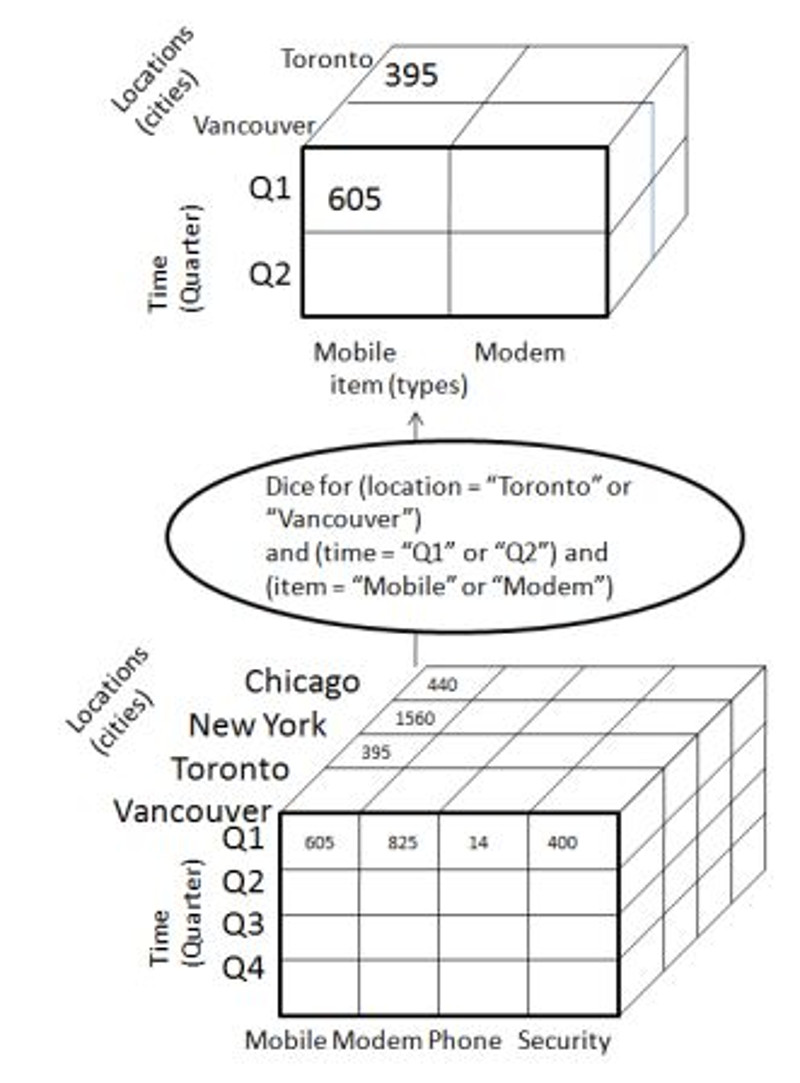
\includegraphics[scale=0.4]{dice}
        \caption{Operación Dice} \cite{operaciones}
        \label{dice}
      \end{center}
    \end{figure}
    
    \begin{figure}
      \begin{center}
        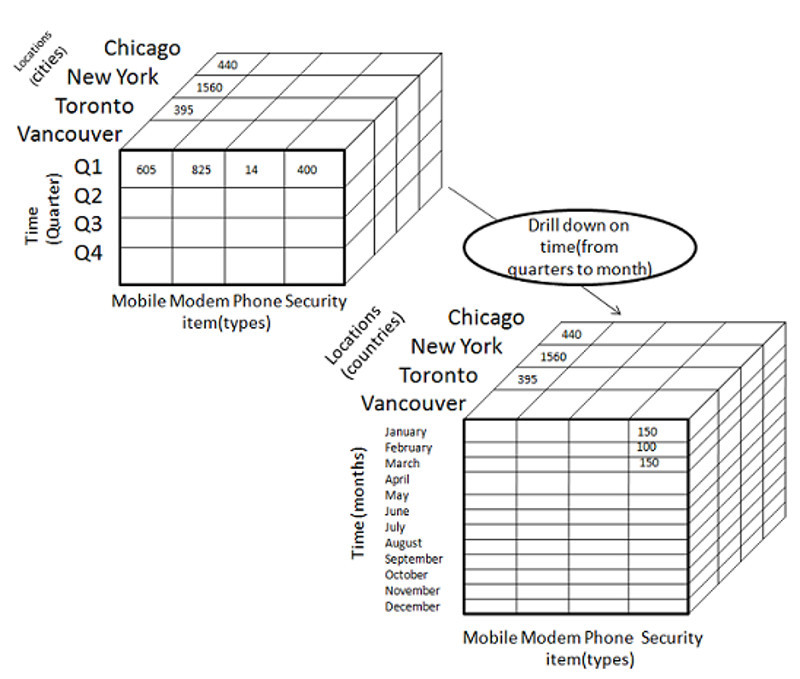
\includegraphics[scale=0.8]{drill_down}
        \caption{Operación Drill Down} \cite{operaciones}
        \label{drill_down}
      \end{center}
    \end{figure}
    
    \begin{figure}
      \begin{center}
        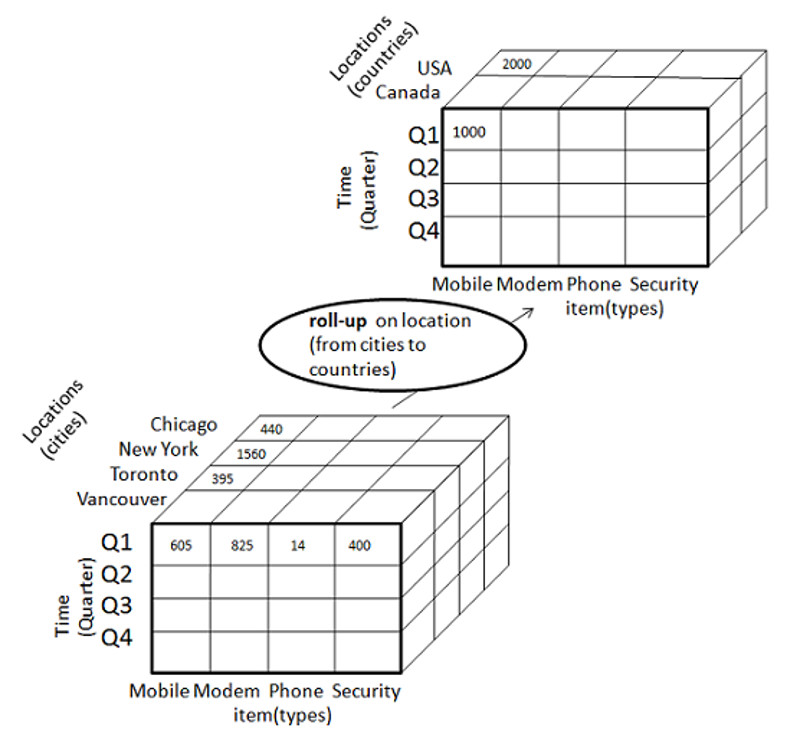
\includegraphics[scale=0.4]{drill_up}
        \caption{Operación Drill Up} \cite{operaciones}
        \label{drill_up}
      \end{center}
    \end{figure}
    
    \begin{figure}
      \begin{center}
        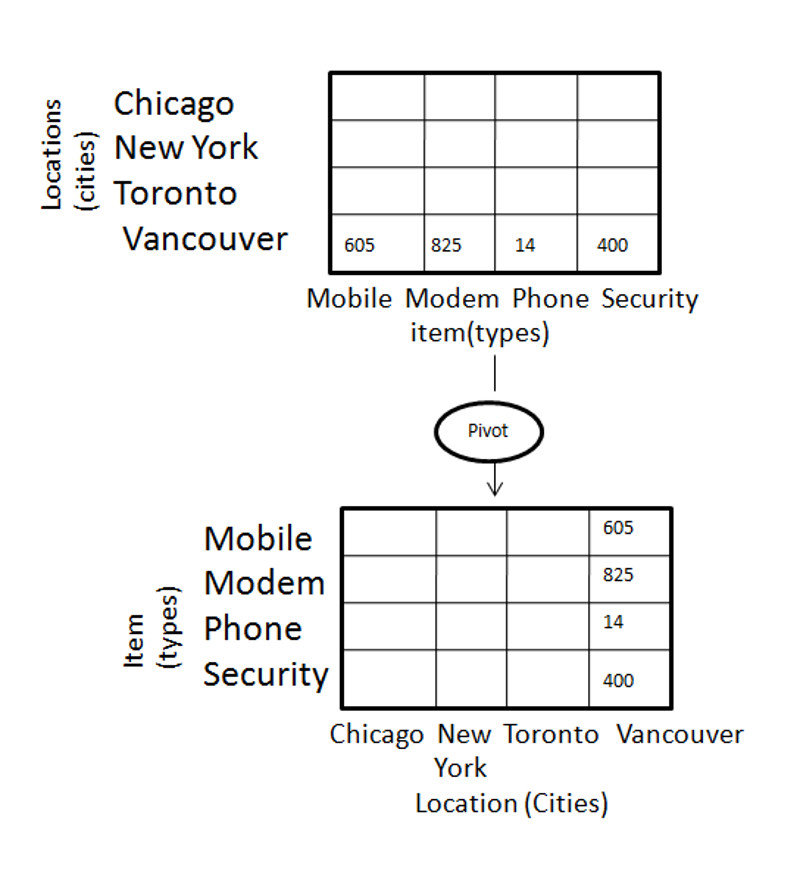
\includegraphics[scale=0.4]{pivot}
        \caption{Operación Pivot} \cite{operaciones}
        \label{pivot}
      \end{center}
    \end{figure}
    
    
    \vspace{0.3in}
    \subsection{Tipos de OLAP}
    
    \subsubsection{ROLAP}
    
    El \textbf{ROLAP} (acrónimo de Relational OnLine Analytical Processing), cuya traducción al castellano es \textbf{Procesamiento Analítico
    Relacional En Línea}, consiste en sistemas y herramientas OLAP construidas sobre una base de datos relacional. Al trabajar con ROLAP se deben
    tener en cuenta las siguientes ventajas y desventajas:
    
    \begin{itemize}
      \item \textbf{Ventajas:}
        \begin{itemize}
          \item Existe una gran variedad de herramientas de carga de datos para sistemas relacionales. Con ésto se consigue que los tiempos de carga
          sean, generalmente, mucho menores que con las cargas MOLAP (lo cual se definirá a continuación) automatizadas.
          \item Los datos se almacenan en una base de datos relacional estándar que puede ser accedida por cualquier herramienta de generación de
          informes SQL (reporting).
        \end{itemize}
      \item \textbf{Desventajas:}
        \begin{itemize}
          \item Muchos desarrolladores de modelos dimensionales ROLAP ignoran el paso de creación de tablas agregadas, con lo cual el rendimiento de
          una consulta se ve afectado debido a la necesidad de consultar las tablas con datos más detallados. Ésto puede evitarse parcialmente
          añadiendo tablas agregadas, sin embargo no es práctico crear tablas agregadas para todas las combinaciones posibles de dimensiones/atributos.
          \item Los sistemas ROLAP se construyen sobre bases de datos de propósito general, por lo que hay algunas funcionalidades especiales, propias
          de las herramientas MOLAP, que no están disponibles en los sistemas ROLAP (tales como el indexado jerárquico especial). Sin embargo, las
          herramientas ROLAP modernas suplen estas carencias con las continuas mejoras del lenguaje SQL, tales como los operadores CUBE y ROLLUP, las
          vistas de cubo DB2, así como otras extensiones SQL OLAP. Estas mejoras SQL pueden mitigar en cierto nivel las diferencias frente a las
          herramientas MOLAP.
          \item Dado que las herramientas ROLAP se basan en SQL para todos sus cálculos, no son apropiadas cuando el modelo realiza muchos cómputos que
          no una traducción simple al SQL (por ejemplo: presupuestos, asignaciones, informes financieros y otros escenarios).
        \end{itemize}
    \end{itemize}
    
    En la Figura \ref{rolap} se puede observar como sería una estructura utilizando una herramienta ROLAP.
    
    \begin{figure}
      \begin{center}
        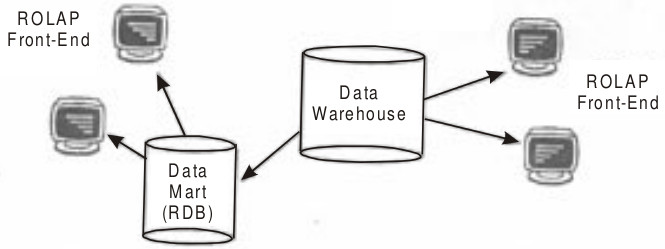
\includegraphics[scale=0.4]{rolap}
        \caption{Estructura de DW utilizando ROLAP} \cite{nagabhushana} Pag. 81.
        \label{rolap}
      \end{center}
    \end{figure}
    
    \subsubsection{MOLAP}
    
    El \textbf{Procesamiento Analítico Multidimensional En Línea} (más conocido por las siglas \textbf{MOLAP}) son las herramientas que ejecutan sus
    cálculos sobre una base de datos multidimensional (MDDB) y por lo cual tienen algunas características a favor y otras en contra.
    
    \begin{itemize}
      \item \textbf{Ventajas:}
        \begin{itemize}
          \item Consultas rápidas debido a ciertas optimizaciones de rendimiento, indexación multidimensional y memoria caché.
          \item Ocupa menor tamaño en disco en comparación con los datos almacenados en base de datos relacional debido a técnicas de compresión.
          \item Automatización del procesamiento de los datos agregados de mayor nivel.
          \item Muy compacto para conjuntos de datos de pocas dimensiones.
        \end{itemize}
      \item \textbf{Desventajas:}
        \begin{itemize}
          \item La etapa de procesamiento (carga de datos) puede ser bastante larga, sobre todo para grandes volúmenes de datos. Normalmente, esto se
          puede evitar con un procesamiento incremental, es decir, sólo procesar los datos que han cambiado (por lo general, datos nuevos) en lugar de
          reprocesar todo el conjunto de datos.
          \item Las herramientas MOLAP tradicionalmente tienen dificultades para consultar modelos con muchas dimensiones.
        \end{itemize}
    \end{itemize} 
    
    \begin{figure}
      \begin{center}
        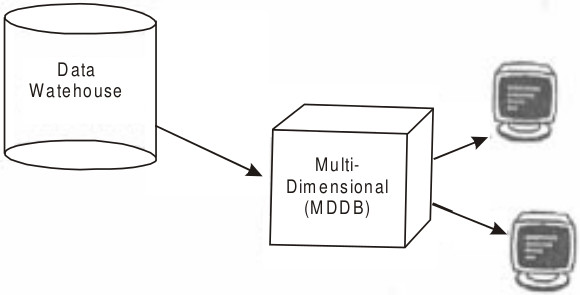
\includegraphics[scale=0.4]{molap}
        \caption{Estructura de DW utilizando MOLAP} \cite{nagabhushana} Pag. 81.
        \label{molap}
      \end{center}
    \end{figure}
    
    En la Figura \ref{molap} se puede observar un ejemplo de estructura modalando la realidad con una herramienta MOLAP.
    
    \subsubsection{HOLAP}

    El coste adicional de los procesos ETL para migrar datos a una herramienta MOLAP y el pobre rendimiento de consulta en los sistemas ROLAP ha generado que la
    mayoría de las herramientas comerciales OLAP usen un modelo \textbf{HOLAP (Hybrid OnLine Analytical Processing)}, el cual permite al diseñador del sistema
    decidir qué porción de los datos serán almacenados en modo multidimensional (MOLAP) y qué porción en modo relacional (ROLAP). Al combinar ambas herramientas
    se obtiene la reducción de los tiempos que demanda la carga de datos (ROLAP) y las optimizaciones en cálculos complejos, lo que beneficia a la fluidez de la
    navegación de los datos (MOLAP). En la Figura \ref{holap} se presenta un esquema modelado con una herramienta HOLAP, donde se puede observar como, dentro de
    una misma arquitectura de DW, conviven ambas tecnologías.
    
    \begin{figure}
      \begin{center}
        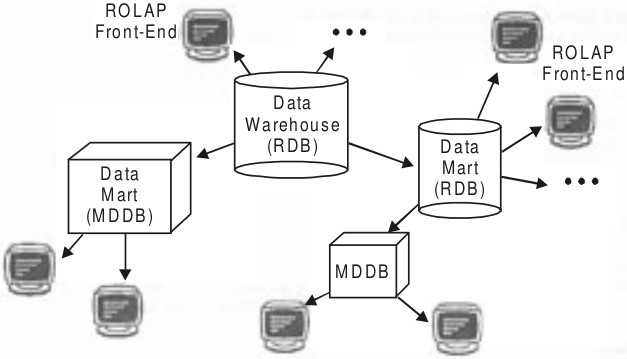
\includegraphics[scale=0.4]{holap}
        \caption{Estructura de DW utilizando HOLAP} \cite{nagabhushana} Pag. 82.
        \label{holap}
      \end{center}
    \end{figure}
    
    
    
    \section{Estado del arte}
    
    En las siguientes secciones se desarrollaran temas que se encuentran actualmente en investigación. Los mismos fueron seleccionados por los autores
    debido a la calidad de información que aportan y, en algunos casos, a la relación que se establece entre las bases de datos y temas afines la
    Inteligencia Artificial.
    
    \subsection{Diseño de un Data Warehouse} 
    
    
    \subsection{Ontologías para la creación de un Data Warehouse}
    
    Como se menciona en \cite{ontologias}, la utilización y el análisis de datos no estructurados como pueden ser los archivos de texto, la web
    semántica, etc., han sido incluidos entre las posibles fuentes de datos, debido a la variedad y cantidad de información que pueden aportar. Lo que
    se intenta conseguir es una forma de automatizar la creación de un DW teniendo como base una ontología. Notar que la misma debe tener una
    estructura tal que contenga la información necesaria para la toma de decisiones, con lo cual las distintas clases estarán relacionadas de forma
    que, terminado el algoritmo, se podrán observar las dimensiones y los hechos del DW. Se utilizará como entrada una ontología (escrita en OWL o RDF)
    para luego obtener un DW.\par
    
    Antes de centrar la atención en el algoritmo propiamente dicho, se repasarán algunos conceptos de la teoría de ontologías que resultan fundamentales
    para la comprensión del tema que se analizará en breve:
    
    \begin{itemize}
      \item \textbf{Object Property:} Las propiedades de objetos son relaciones entre instancias de 2 clases. Por ejemplo, ownedBy, podría ser una
      object property con la clase Vehículo como dominio y la clase Persona como rango, la misma establece la relación de pertenencia de un vehículo a
      una persona.
      \item \textbf{Data Property:} Las propiedades de datos son como las object properties pero tienen como dominio una clase y como rango un tipo de
      datos\footnote{Una instancia de una data property relaciona un individuo de la clase dominio con un valor concreto del tipo de datos del rango}.
      Por ejemplo si a una persona se le quisiera asignar el nombre completo, entonces se puede definir la data property fullName con dominio en Person
      y rango string.
      \item \textbf{Individials:} Los individuos de una ontología representan los objetos o instancias de las clases definidas en la misma.
    \end{itemize}
    
    
    Habiéndose presentado las anteriores definiciones, se procederá a detallar el algoritmo en cuetión. El mismo consta de las siguientes etapas:
    
    \begin{itemize}
      \item \textbf{Creación de tablas}
      \item \textbf{Detección de relaciones de subclase}
      \item \textbf{Definir relaciones a partir de propiedad de objetos}
      \item \textbf{Definir relaciones a partir de propiedad de datos}
      \item \textbf{Insertar datos en las tablas}
    \end{itemize} 
    
    \subsubsection{Creación de tablas}
    
    En esta primer etapa el objetivo es que para cada clase en la ontología se deberá crear una tabla en el DW. Es decir, al navegar toda la ontología,
    cada vez que se encuentre una clase, se debe crear una tabla con el mismo nombre en el DW. En la Figura \ref{createTables} se describen, con un
    diagrama de flujo, los pasos a seguir.
    
    \begin{figure}
      \begin{center}
        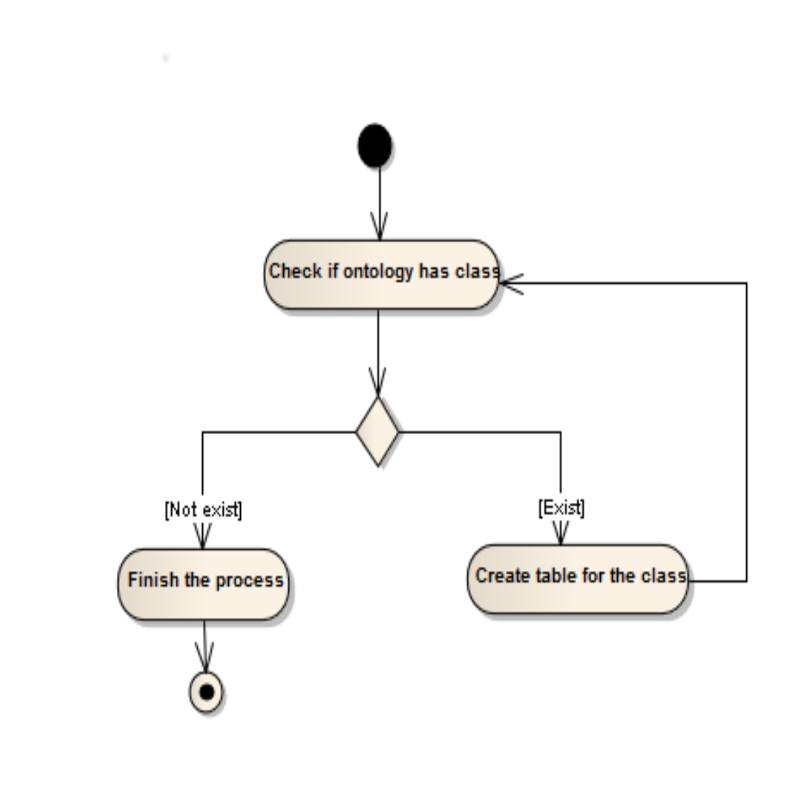
\includegraphics[scale=0.6]{create_tables}
        \caption{\textbf{Primer etapa:} Creación de tablas} \cite{ontologias} Pag. 20.
        \label{createTables}
      \end{center}
    \end{figure}
    
    \subsubsection{Detección de relaciones de subclase}
     
    Ahora se debe centrar la atención en buscar relaciones entre clases del tipo \textbf{subclaseDe}, también conocidas como \textbf{Es\_Un}. Estas
    relaciones expresan que una determinada clase es subclase de otra más abstracta. La subclase hereda todas las propiedades de su clase padre.
    Entonces, cuando se navega toda la ontología y se encuentra este tipo de relación entre dos clases, se tiene que crear una clave foránea (foreing
    key) en la tabla padre y generar una relación uno a muchos entre ambas tablas. Para comprender mejor esta instancia del algoritmo observese la
    Figura \ref{subClase}.
   
    \begin{figure}[!htb]
      \begin{center}
        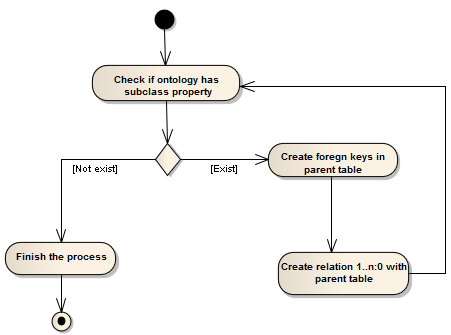
\includegraphics[scale=0.6]{sub_clase}
        \caption{\textbf{Segundo etapa:} Detección de relaciones de subclase} \cite{ontologias} Pag. 20.
        \label{subClase}
      \end{center}
    \end{figure}
     
     
    \subsubsection{Definir relaciones a partir de propiedad de objetos}
    
    Se recorre la ontología en busca de propiedades de objetos. Este tipo de propiedades tienen asociadas un dominio y un rango, los cuales son clase
    (representados con tablas en el DW). Teniendo las tablas dominio y rango, se genera, para cada propiedad de objeto, una relación uno a muchos entre ambas. En
    el caso en que no existan el dominio y el rango (debido a estar tratando con una sub-propiedad), se toma el dominio y el rango de la propiedad padre y se
    realiza el mismo procedimiento. Se puede observar en la Figura \ref{objectProperty} qué pasos son los que se deben realizar para completar correctamente esta
    etapa.
    
    \begin{figure}[!htb]
      \begin{center}
        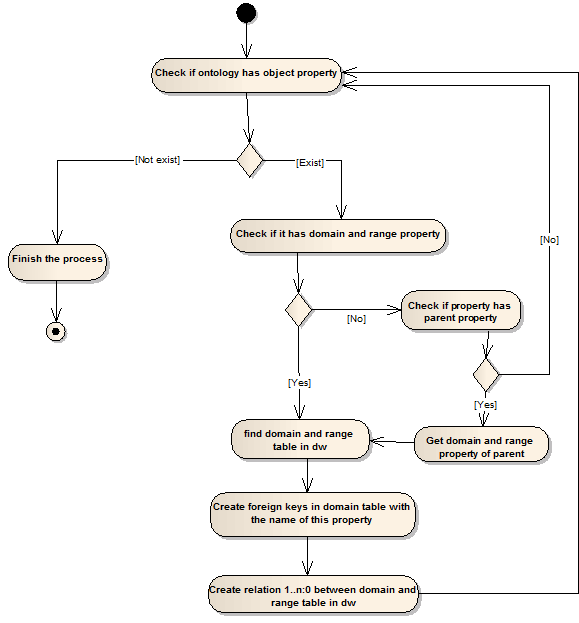
\includegraphics[scale=0.6]{object_property}
        \caption{\textbf{Tercer etapa:} Detección de propiedades de objeto} \cite{ontologias} Pag. 21.
        \label{objectProperty}
      \end{center}
    \end{figure}
    
    
    \subsubsection{Definir relaciones a partir de propiedad de datos}
    
    Se buscan todas la propiedades de datos en la ontología. Las propiedades de datos vinculan una clase con un tipo de dato específico. Similar a las propiedades
    de objetos, las propiedades de datos tienen dominio y rango. Si se puede identificar el dominio y rango de la propiedad, en la tabla que representa al dominio
    creamos una columna con el mismo nombre de la propiedad y seteamos el tipo de esa columna como el rango de la propiedad. En caso que no se pueda encontrar el
    dominio y rango, se debe intentar identificar la propiedad padre de esta propiedad (si existe) y dado el caso, realizamos el mismo procedimiento con el
    dominio y rango de la propiedad padre. Se puede apreciar, en la Figura \ref{dataProperty}, qué es lo que se debe realizar en esta etapa.
    
    \begin{figure}[!htb]
      \begin{center}
        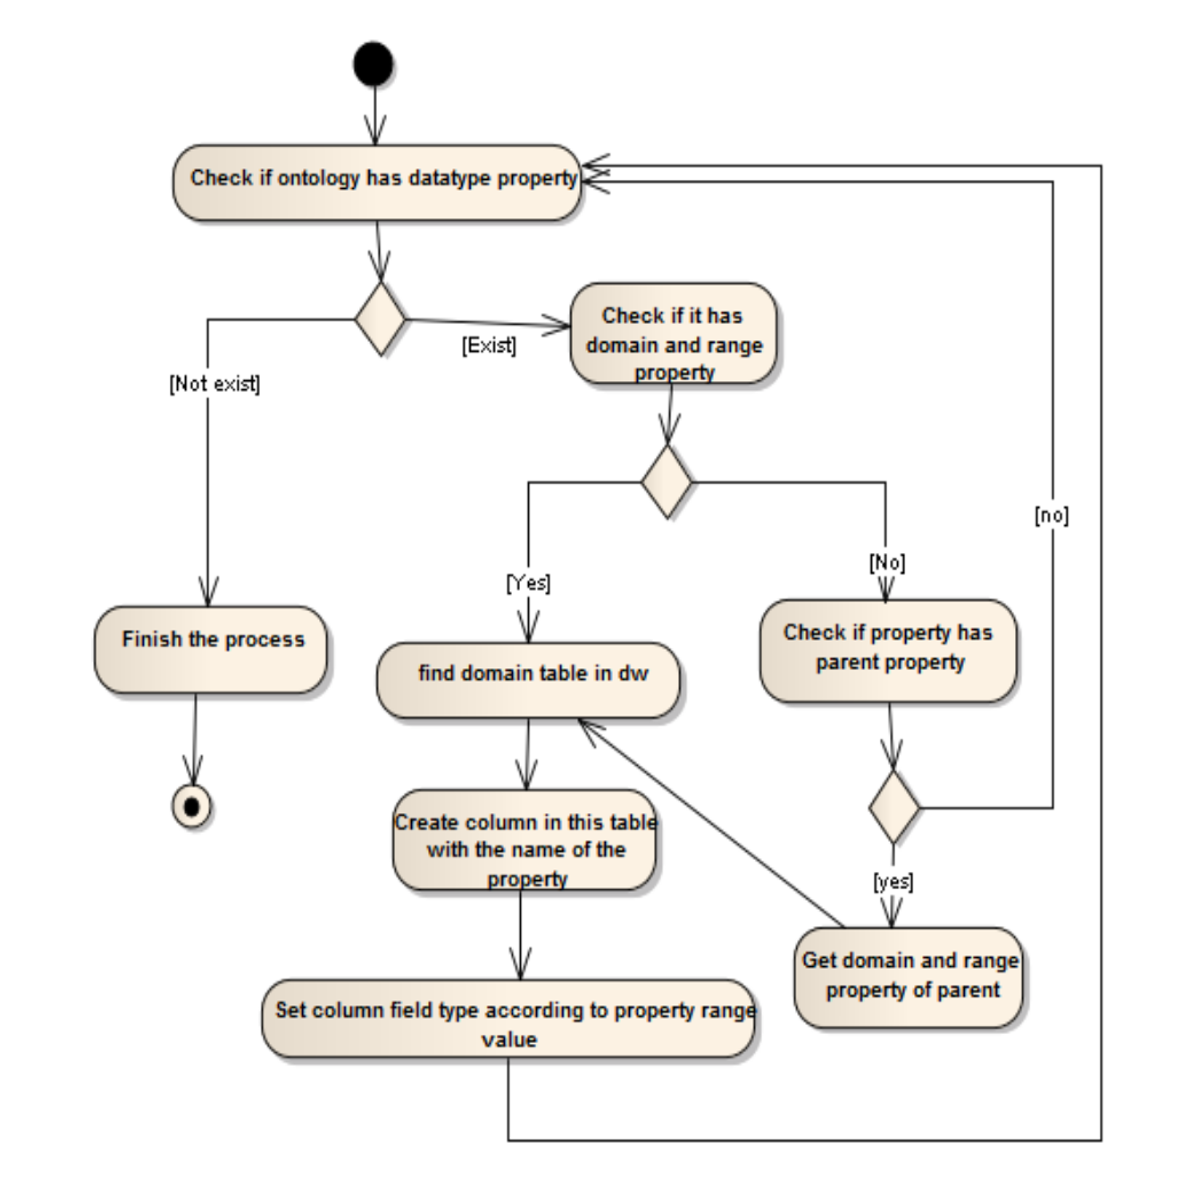
\includegraphics[scale=0.6]{data_property}
        \caption{\textbf{Cuarta etapa:} Detección de propiedades de dato} \cite{ontologias} Pag. 21.
        \label{dataProperty}
      \end{center}
    \end{figure}
    
    
    \subsubsection{Insertar datos en las tablas}
    
    En este punto es necesario enfocar la atención en los individuos de la ontología. Cada individuo se corresponde con una clase en particular, por lo tanto se
    insertará un nuevo registro (creando así un nuevo id) que será la representación del individuo en el DW. Luego, si existe alguna clase padre con respecto a la
    que se acaba de hacer el insert, se insertará un nuevo registro en la misma, el cual tendrá relacionado la clave ajena correspondiente. Como siguiente paso,
    se deben tener en cuenta las propiedades de datos. Se busca la tabla correspondiente a la clase dominio de la propiedad y se actualiza la columna que tiene el
    mismo nombre que la propiedad con el valor del rango según el individuo respectivo del dominio. En caso que no exista la clase dominio, se busca la clase
    dominio de la propiedad de datos padre. De forma similar, teniendo en vista las propiedades de objetos,  se identifica la tabla dominio (en su defecto, la 
    tabla dominio de la propiedad padre) y se actualiza la fila correspondiente al individuo de la clase dominio, en la columna con el mismo nombre que la
    propiedad, con el valor del individuo de la clase rango. En caso que no exista la columna en la tabla dominio, ésta es creada y se realiza el procedimiento
    antes descripto. El diagrama de la Figura \ref{insertingData} ilustra de forma más detallada lo recien explicado, incluyendo cada uno de los pasos a seguir.
    
    \begin{figure}[!htb]
      \begin{center}
        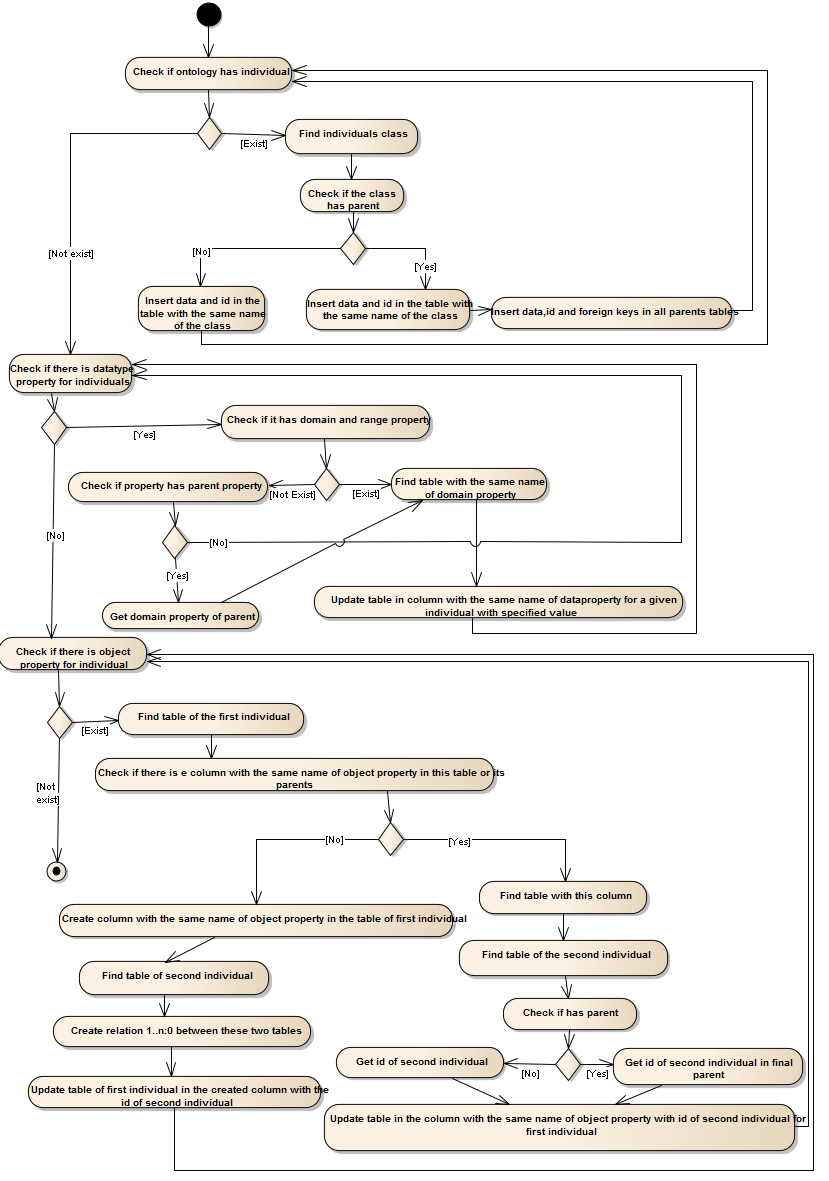
\includegraphics[scale=0.4]{inserting_data}
        \caption{\textbf{Quinta etapa:} Inserción de datos} \cite{ontologias} Pag. 22.
        \label{insertingData}
      \end{center}
    \end{figure}
    
    
    Como se puede apreciar, haciendo uso de cada una de las etapas anteriormente explicadas, se puede obtener una estructura dimensional, la cual estará
    formada por tablas de dimensiones y de hechos, a partir de datos organizados utilizando OWL. Cabe remarcar que cada una de las etapas tiene una manera
    mecánica de realizarse, con lo cual, facilita la tarea y, por otro lado, permite la automatización de ciertas partes del método utilizando algoritmos con el
    fin de simplificar aún más la labor a realizar.
    
    \subsection{Fuzzy Data Warehouse}
    
    
    \subsection{Web Warehouse}
    
    \subsubsection{Motivación}
    
    Un \textbf{Web Warehouse} es un DW, en el cual la información es obtenida de las posibles fuentes de datos de la web. Como se menciona en \cite{webwarehouse}
    la idea de Web Warehouse es algo similar a la de un DW ya que en su arquitectura ya son bastante parecidos. La calidad de los datos es un punto crucial a la
    hora de utilizar datos provenientes de la web debido a que pueden ser poco relevantes, erróneos en sus tipos de datos, estar incompletos y tener valores
    nulos. En \cite{webwarehouse} se plantean una arquitectura y el ciclo de vida del WW con el fin de tener flexibilidad a la hora de elección de las fuentes de
    datos y llevar un buen control de los datos utilizados.
    
    
    \subsubsection{Arquitectura}
    
    La arquitectura del WW se puede dividir en algunos módulos, cada uno de ellos con tareas específicas:
    
    \begin{itemize}
      \item \textbf{Módulo DSI:} De la sigla en ingles Data Service Infrastructure (ó infraestructura de servicio de datos). Este módulo tiene 3 tareas
      principales:
        \begin{itemize}
          \item Proveer un mecanismo para extraer datos de los diferentes tipos WDS (Web Data Source ó, su traducción al castellano, fuentes de datos web) y
          mostrarlos a todos ellos como DS homogéneos (Data Service ó servicio de datos). Los DS son los encargados de acceder y extraer la información de la web.
          \item Monitorear los DS y periódicamente controlar la calidad de los datos que ingresan. Estos controles son realizados por ciertos DS que son
          invocados por el móludo QM (Quality Measurement ó de medición de calidad) e incluyen el almacenamiento de metadatos de DQ (Data Quality ó calidad de
          datos) y QoS (Quality of Service ó calidad de servicio).
          \item Provee mecanismos para reaccionar ante la degradación de un DS, ya que si ésto sucede, los datos perderán relevancia.
        \end{itemize}
      \item \textbf{Módulo integrador:} Este módulo lleva a cabo la integración de datos y provee los mismos en un formato normalizado, construyendo con ellos la
      IDB (Integrated Data Base ó base de datos integrada). Sus principales objetivos son la selección de los DS con el fin de obtener calidad en los datos
      extraidos de la web, integración de datos y la generación de metadatos de esos datos integrados.
      \item \textbf{Módulos ETL y OLAP:} Estos módulos realizan las tareas usuales salvo que deben propagar los metadatos de la calidad de datos.
      \item \textbf{Módulo DWQM:} Es la sigla para Data Warehouse Quality Measurement ó medición de calidad del DW. Como lo indica su nombre, es el módulo
      encargado de medir la calidad de los datos del DW.
    \end{itemize}
    
    Las conexiones entre los distintos módulos pueden ser observadas en la Figura \ref{ww_arq}, donde se puede apreciar claramente la propagación entre de los
    metadatos (punto destacado en la explicación de los módulos).
    
    \begin{figure}[!htb]
      \begin{center}
        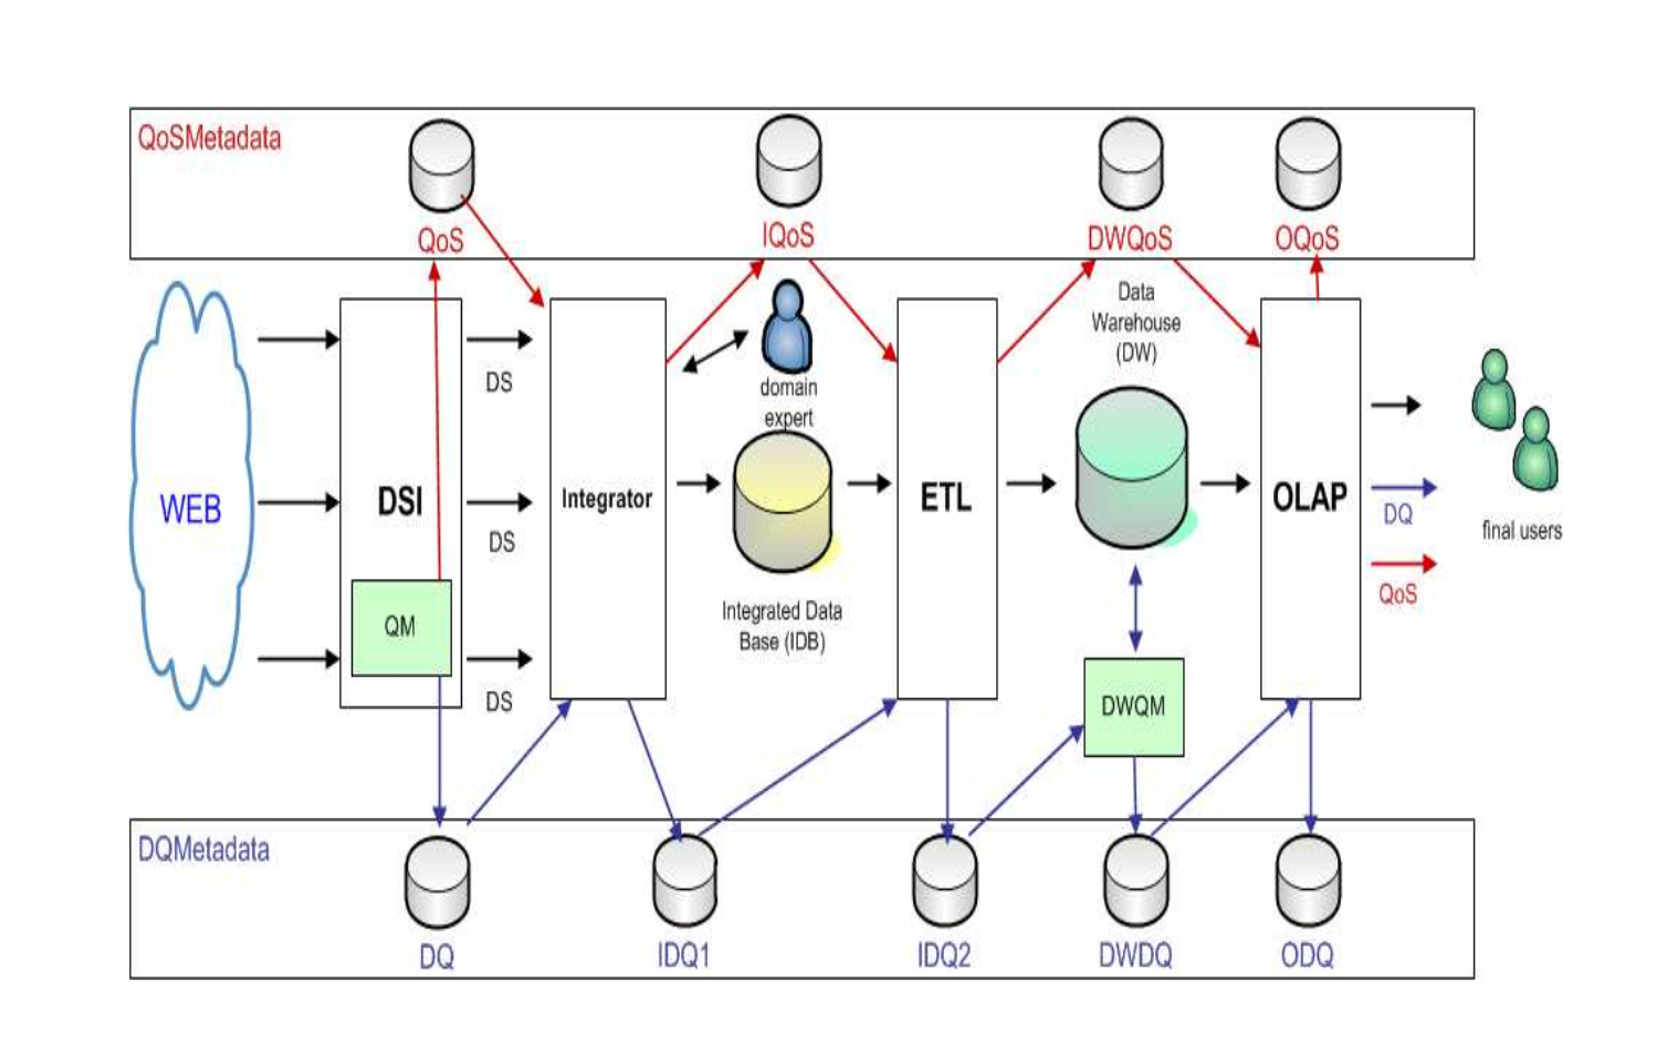
\includegraphics[scale=0.25]{ww_arq}
        \caption{Arquitectura genérica de un Web Warehouse} \cite{webwarehouse} Pag. 2.
        \label{ww_arq}
      \end{center}
    \end{figure}
    
    
    \subsubsection{Ciclo de vida de un WW}
    
    El ciclo de vida de un WW, está compuesto por distintas etapas y en el se presentan los roles de las personas que participan en cada una. Las
    etapas son las que se muestran en la Figura \ref{lifecycle} y detalladas a continuación:
    
    \begin{figure}[!htb]
      \begin{center}
        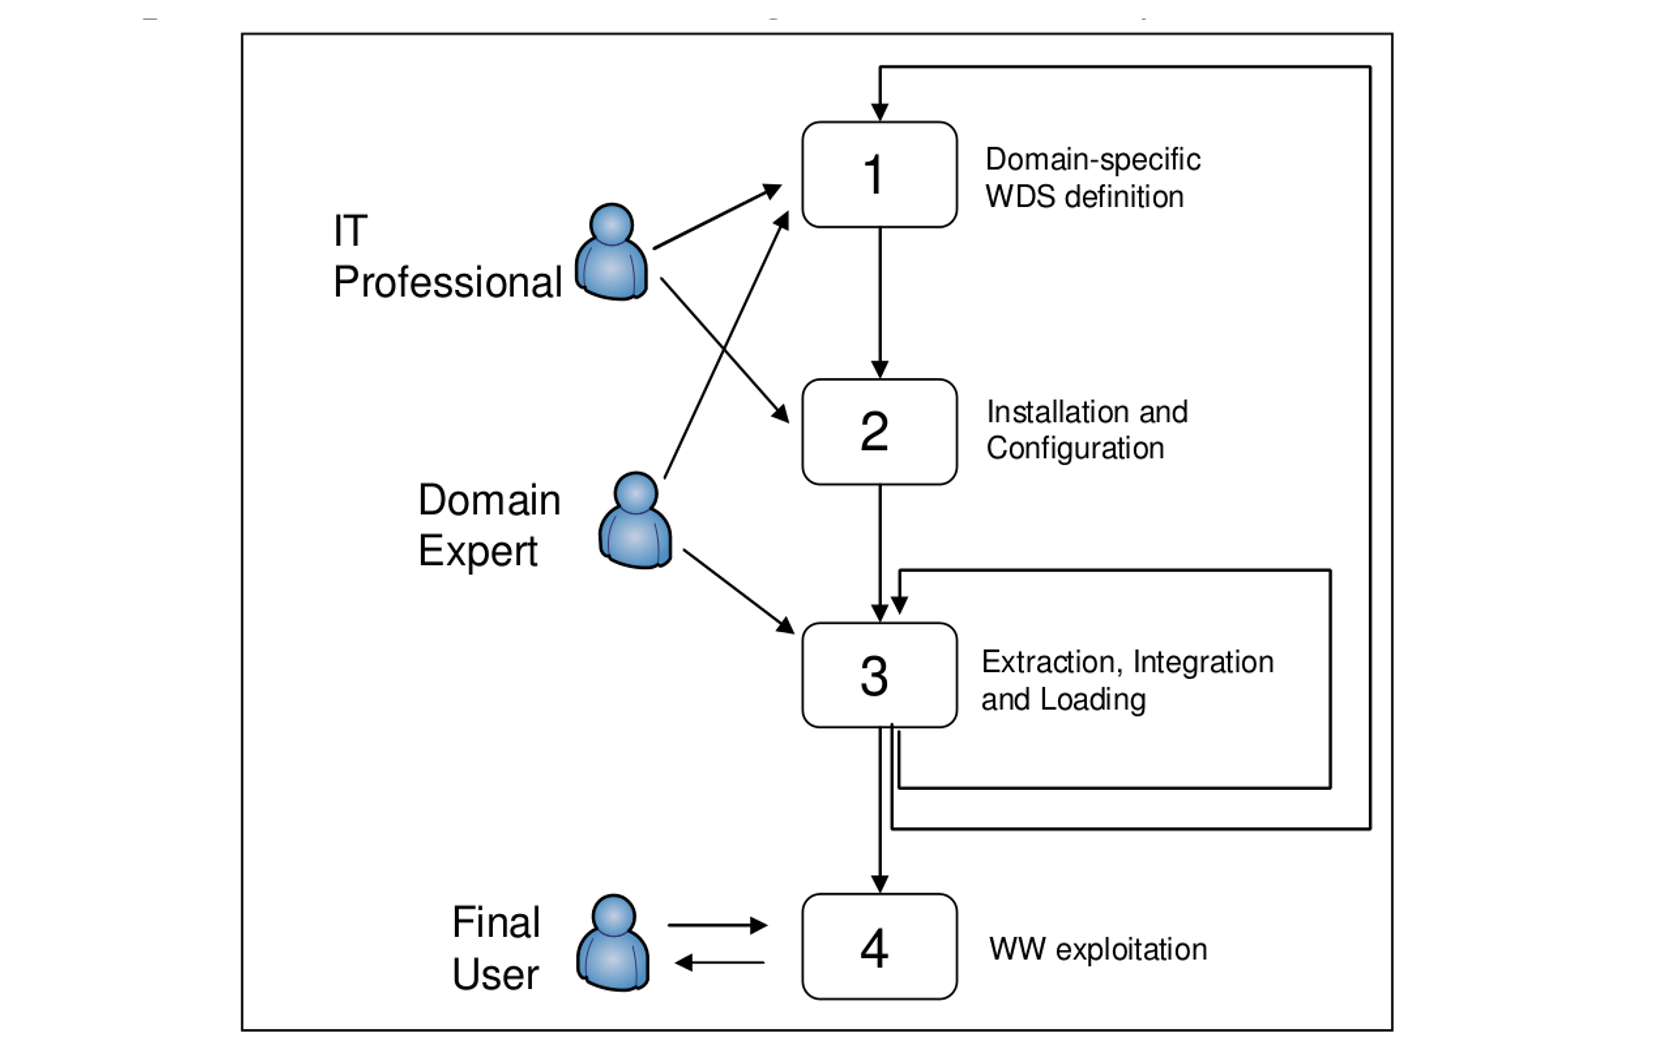
\includegraphics[scale=0.25]{lifecycle}
        \caption{Ciclo de vida de un Web Warehouse} \cite{webwarehouse} Pag. 3.
        \label{lifecycle}
      \end{center}
    \end{figure}
    
    \begin{enumerate}
      \item En este paso se elige las fuentes de datos web específicas para el dominio en el que se está trabajando, teniendo en cuenta la calidad de las mismas.
      Estas fuentes se llaman WDS seleccionadas.
      \item La siguiente instancia es donde se hacen la instalación y configuración de la plataforma para el dominio determinado dependiendo de sus
      requerimientos. Consiste en las siguientes tareas:
        \begin{enumerate}
          \item Diseño y definición del DW, lo que incluye el esquema del mismo y los procesos ETL
          \item Diseño del esquema del DSI
          \item Desarrollo de los DS
          \item Selección de los DS
        \end{enumerate}
      \item Aquí es donde se da la extracción, integración, transformación y carga de datos controlando la calidad de los mismos. En esta etapa es cuando los
      datos se toman de la web, pasan a través del sistema y cargan el DW. Como se ve en la Figura \ref{lifecycle}, desde esta etapa se puede volver a la
      primera, lo cual puede darse en el caso que se quisiera agregar una nueva fuente de datos como pueden ser nuevos sitios web. La calidad de los datos sigue
      siendo de vital importancia.
      \item Esta etapa es en la que se realiza la explotación de los datos por el usuario final.
    \end{enumerate}
    
    
    \subsubsection{Calidad de datos}
    
    Como se ha estado mencionando, la calidad de los datos es uno de los puntos más importantes en la arquitectura de un WW, ya que es la que define la calidad
    de toda la solución de negocios que se está ofreciendo al cliente u organización. Para que el lector tenga una idea más concreta sobre la calidad de los
    datos se plantean 6 factores que, a juzgar por los autores, engloban todos los aspectos referentes al tema, los cuales son:
    
    \begin{itemize}
      \item \textbf{Presición:} Sintáctica y semánticamente correctos.
      \item \textbf{Completitud:} Cuan densos son los datos, es decir, cuanto cubren de todo lo que se necesita.
      \item \textbf{Frescura:} Periodicidad con que se cargan los datos, límite de tiempo luego del cual los datos dejan de ser válidos.
      \item \textbf{Consistencia:} Los datos deben ser consistentes respecto del dominio en que se trabaja.
      \item \textbf{Unicidad:} No debe haber duplicidad en los datos.
      \item \textbf{Confiabilidad:} Los datos deben tener credibilidad y ser objetivos.
    \end{itemize}
    
    
  %\end{flushleft}

  \vspace{10in}

  % ############################ INICIO BIBLIOGRAFIA ############################

\printbibliography

%   \begin{thebibliography}{9}
%     
%     \bibitem{hefestov2}
%     [Bernabeu, 2010] Ing. Bernabeu Ricardo Dario.
%     \textit{HEFESTO: Metodología para la Construcción de un Data Warehouse}.
%     
%     \bibitem{dim_models}
%     Modelos dimensionales.
%     \textit{http://www.dataprix.net/node/16678}
%     
%     \bibitem{nagabhushana}
%     [Nagabhushana, 2006] S. Nagabhushana.
%     \textit{Data Warehousing: OLAP and Data Mining}.
%     
%     \bibitem{olap_solutions}
%     [Thomsen, 2006] Erik Thomsen.
%     \textit{OLAP Solutions: Building Multidimensional Information Systems. Second edition}.
%     
%     \bibitem{agg_tables}
%     Pentaho Mondrian Documentation.
%     \textit{http://mondrian.pentaho.com/documentation/aggregate\_tables.php}
%     
%     \bibitem{operaciones}
%     Operaciones OLAP.
%     \textit{http://www.tutorialspoint.com/dwh/dwh\_olap.htm}
%     
%     \bibitem{ontologias}
%     [Talebzadeh, 2014] Shiva Talebzadeh, Mir Ali Seyyedi, Afshin Salajegheh.
%     \textit{Automated Creating a Data Warehouse from Unstructured Semantic Data}.
%     
%     \bibitem{webwarehouse}
%     [Marotta, 2012] Adriana Marotta, Laura González, Raúl Ruggia.
%     \textit{A Quality Aware Service-oriented Web Warehouse Platform}.
%     
%   \end{thebibliography}
  
  % ############################ FIN BIBLIOGRAFIA ############################
  
  
  \printindex
  
\end{document}
